%\documentclass[12pt]{scrreprt}
\documentclass[12pt]{report} 

% language may be romanian or english (default is english)
% type may be bachelor or master (default is bachelor)
\usepackage[language=english, type=bachelor]{style}

%\geometry{a4paper,top=2.5cm,left=3cm,right=2.5cm,bottom=2.5cm}
%in style
%controlling the appearance of your headers and footers
\usepackage{amsmath}
\usepackage{amssymb}
\usepackage{microtype}
\usepackage{tikz}
\usetikzlibrary{arrows, positioning, shapes.geometric}
\usepackage{csquotes}
\usepackage{fancyhdr}
\pagestyle{fancy}
\setlength{\headheight}{14.5pt}
\lhead{}
\chead{}
\renewcommand{\headrulewidth}{0.2pt}
\renewcommand{\footrulewidth}{0.2pt}

% Allow LaTeX more flexibility breaking long paragraphs to avoid overfull hboxes.
\emergencystretch=2em

\begin{document}

\specialization{Artificial Intelligence}	
\title{Real-Time Intrusion Detection for Web Applications Using Deep Learning}					   
\author{Rares Marta}											
\supervisor{Alexandra--Ioana Albu}				
				
\maketitle


\newpage
\thispagestyle{empty}
\mbox{}
\newpage
\pagenumbering{roman} 

\cleardoublepage
ABSTRACT
\vspace{0.5cm}	
\hrule
\vspace{0.5cm}	

This thesis aims to design and implement a real-time intrusion detection system capable of analyzing web traffic and identifying malicious behavior using deep learning methods. The work is situated at the intersection of artificial intelligence and cybersecurity and focuses on building a practical system that can operate in a controlled web environment.

The thesis will include a study of the relevant literature in intrusion detection, machine learning, and deep learning for cybersecurity, with particular attention to approaches designed for traffic classification and malicious behavior detection. It will also analyze the challenges involved in evaluating such systems, especially with respect to realism, model generalization, and real-time deployment constraints.

The practical component of the thesis will consist of data processing, model training and evaluation, and the implementation of a demonstration environment in which traffic generated in a controlled web setting is monitored and classified in real time. The originality of the project is expected to come from combining deep learning-based intrusion detection with an interactive demonstration platform that highlights real-time monitoring and alert generation.

\tableofcontents


\newpage
\pagenumbering{arabic}

\chapter{Introduction}
\label{chap:introduction}

\section{Context and Motivation}
\label{sec:intro_motivation}

\par Intrusion Detection Systems (IDS) are a core defensive layer in modern networks, monitoring traffic to detect malicious behaviour such as denial-of-service attacks, reconnaissance scans, brute-force attempts, and data exfiltration. The classical approach is signature-based detection, in which traffic is matched against a database of hand-written rules describing known attacks; the widely deployed Snort system is the canonical example \cite{Roesch1999}. Signature matching is fast and precise on threats it already knows, but it has two structural weaknesses: it cannot recognise an attack for which no rule has been written, and the rule set must be maintained by hand as new threats appear.

\par These weaknesses have become more pressing with the growth of the Internet of Things (IoT). Modern deployments place large numbers of constrained, infrequently patched devices on the same networks as critical services, and the volume and diversity of the resulting traffic strain a detection model that depends on enumerating every attack in advance. The same devices are attractive targets: compromised IoT endpoints are routinely conscripted into large botnets and used to launch volumetric denial-of-service campaigns, which is reflected in benchmark data where denial-of-service and distributed denial-of-service flows dominate the attack distribution \cite{CICIoT2023}.

\par Machine learning, and deep learning in particular, offers an alternative that learns the statistical structure of traffic directly from data rather than from hand-written rules \cite{Ferrag2020, Lansky2021}. A model trained on labelled flows can, in principle, generalise to variants of known attacks and flag anomalous behaviour without an exact signature. This premise has produced a large literature reporting strong benchmark accuracy for neural intrusion detection, including work that applies deep models to real-time web intrusion detection rather than offline analysis alone \cite{AIIDS2020, Wu2022}.

\section{The Research-to-Deployment Gap}
\label{sec:intro_gap}

\par Strong benchmark numbers do not by themselves yield a deployable detector. This thesis addresses the gap between the two \cite{Apruzzese2023}. Three issues recur. First, many reported results are obtained on random train/test splits, which let near-duplicate flows from the same capture session appear in both partitions and inflate the measured accuracy relative to what the model would achieve on genuinely unseen traffic. Second, network traffic drifts: attack tooling and benign usage both change over time, so a model evaluated without respect to temporal order is not tested under the conditions it will actually face \cite{Andresini2021}. Third, a deployed detector must do more than emit a label: it must report a confidence that can be trusted, and modern neural networks are known to be systematically overconfident unless their outputs are explicitly calibrated \cite{Guo2017}. To these we add the practical constraint that real-time operation imposes a latency budget an offline benchmark never measures.

\par This thesis builds these concerns into the design from the outset. Evaluation uses a temporally ordered split so that the test set is strictly later than the training data; the deep model is measured against strong tabular baselines under identical conditions so that any claimed advantage is real; the classifier's confidence is calibrated before it is shown to a user; and inference latency is benchmarked as an explicit acceptance criterion.

\section{Approach and Scope}
\label{sec:intro_approach}

\par The work is built on the CICIoT2023 dataset, a large-scale IoT intrusion-detection benchmark of over 46 million labelled flow records spanning 33 attack types, captured in a 105-device smart-home testbed \cite{CICIoT2023}. The primary classifier is a Multi-Layer Perceptron (MLP) trained at two granularities: a binary attack-versus-benign task and an eight-class task over coarse attack families. Because the public CICIoT2023 features are tabular flow statistics rather than raw packets, the deep model is not assumed to be the best tool by default; recent evidence shows that well-tuned simple neural networks are competitive with gradient-boosted trees on tabular data \cite{Kadra2021}, and the thesis tests this empirically by comparing the MLP against Random Forest and XGBoost baselines on the same splits. Beyond offline evaluation, the trained model is deployed behind a live demonstration in which scripted attacks are launched against a controlled target and the resulting flows are classified in near real time.

\par The scope is bounded in two respects. The system is trained and evaluated only on the 39-feature public release of CICIoT2023, which is derived from packet headers and flow metadata and carries no payload features; detection of application-layer attacks, whose signal lies in the payload, is therefore expected to be limited, and the results chapter reports this rather than working around it. Generalisation beyond the smart-home setting of the dataset is not claimed.

\section{Objectives and Contributions}
\label{sec:intro_contributions}

\par The thesis makes six contributions. The first is a reproducible end-to-end pipeline from raw per-folder CICIoT2023 captures to a live per-flow classifier, with deterministic seeding and a fixed artefact contract so that results can be regenerated and the trained model served without re-running training. The second is a temporal evaluation of an MLP against Random Forest and XGBoost baselines at binary and eight-class granularities, reporting accuracy, macro-F1, and weighted-F1 on the train, validation, and test partitions. The third is a feature analysis that identifies the most discriminative flow features and prunes the 39 public features to a 25-feature set, dropping near-zero-variance flags and redundant continuous columns found through variance and correlation analysis. The fourth is confidence calibration of the deep model by temperature scaling \cite{Guo2017}, which lowers the expected calibration error so that the confidence shown to a user reflects empirical accuracy instead of sitting uniformly near certainty. The fifth is a deployed demonstration system, NEURAL IDS, comprising a containerised inference backend and a web dashboard, which validates the core classification functionality against both benign and synthetic-attack traffic. The sixth is an account of where the approach falls short, particularly the eight-class attack-family task, on which no model reaches the 0.85 weighted-F1 bar met on the binary task; this shortfall stems from the fact that the public features describe transport-layer behaviour only.

\section{Thesis Structure}
\label{sec:intro_structure}

\par The remainder of this thesis is organised as follows. Chapter~\ref{chap:theoretical_background} presents the theoretical background, covering intrusion detection systems, deep learning for traffic classification, and the CICIoT2023 dataset. Chapter~\ref{chap:requirements} states the application requirements and specification, defining the problem, the actors involved, and the functional and non-functional constraints the system must satisfy. Chapter~\ref{chap:design_implementation} describes the design, implementation, and testing of the application, including the data pipeline, the model architecture and training procedure, the live-demo environment, and the verification of the core functionality. Chapter~\ref{chap:results} reports the experimental results and discusses the findings. Chapter~\ref{chap:conclusions} concludes the thesis and outlines directions for future work.

\section{Declaration on the Use of Generative AI Tools}
\label{sec:intro_ai_declaration}

\par Generative AI tools were used during the preparation of this thesis. AI-based coding assistants supported the development of the training pipeline and the demonstration application by generating boilerplate code, suggesting refactorings, and helping diagnose errors. AI language models were also used to draft and revise portions of the written text for clarity and concision. All such output was reviewed, tested, and edited by the author. Every experimental result reported here was produced by running the pipeline and was verified independently of any AI tool, and the author takes full responsibility for the content of the thesis, the correctness of the results, and the final wording.

%\addcontentsline{toc}{chapter}{Introduction}

\chapter{Theoretical Background}
\label{chap:theoretical_background}

\par This chapter presents the theoretical foundations underlying the work developed in this thesis. It begins with an overview of intrusion detection systems and their role in network security, then introduces deep learning as a tool for traffic classification, with a focus on multi-layer perceptrons. Finally, it describes the CICIoT2023 dataset, which serves as the training and evaluation basis for the models developed in subsequent chapters.

\section{Intrusion Detection Systems}
\label{sec:ids}

\par An Intrusion Detection System (IDS) is a security mechanism that monitors network traffic or host activity to identify malicious behavior. As networks have grown in scale and complexity, traditional perimeter defenses such as firewalls have proven insufficient on their own: attackers routinely bypass static rules and exploit new vulnerabilities, while modern networks exhibit high throughput, heterogeneity, and continual change \cite{Lansky2021}. IDS complement these defenses by analyzing traffic patterns and flagging suspicious activity.

\par IDS can be broadly categorized into two paradigms based on their detection methodology: signature-based and anomaly-based systems.

\subsection{Signature-Based Detection}
\label{subsec:signature_ids}

\par Signature-based IDS, exemplified by tools such as Snort and Suricata, operate by scanning network traffic for predefined patterns of known malicious activity \cite{Roesch1999}. These signatures can describe byte sequences, header anomalies, or protocol violations. Signature-based systems are highly effective at detecting known attacks with high precision, and they produce few false positives when the signature database is well-maintained.

\par However, their static nature makes them fundamentally limited against novel threats. Zero-day exploits, polymorphic attacks, and previously unseen attack variants will not match any existing signature and will therefore pass undetected. Signature databases also require continuous manual updates to remain effective, which introduces an inherent lag between the emergence of a new attack and the availability of its corresponding signature.

\subsection{Anomaly-Based Detection}
\label{subsec:anomaly_ids}

\par Anomaly-based IDS take a different approach: instead of matching against known attack patterns, they learn a model of normal network behavior and flag deviations from this baseline as suspicious. This paradigm has the significant advantage of being able to detect previously unseen attacks, since any traffic that deviates sufficiently from the learned normal profile will trigger an alert.

\par The trade-off is a higher false positive rate. Unusual but legitimate traffic (such as a sudden spike in usage during a product launch, or an uncommon protocol used by a newly deployed application) can be incorrectly flagged as malicious. The sensitivity of anomaly-based systems depends heavily on the quality of the normal behavior model and on the threshold chosen to separate normal from anomalous activity.

\par Figure \ref{fig:ids_pipeline} illustrates the typical architecture of a real-time deep learning-based IDS, showing the end-to-end pipeline from raw packet capture to alert generation.

\begin{figure}[htbp]
    \centering
    \resizebox{\textwidth}{!}{%
    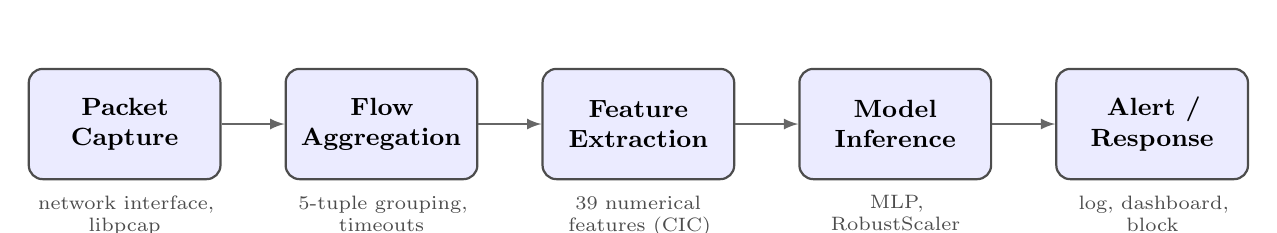
\begin{tikzpicture}[
        node distance=0.8cm,
        stage/.style={
            rectangle,
            rounded corners=5pt,
            draw=black!70,
            fill=blue!8,
            thick,
            minimum width=2.4cm,
            minimum height=1.4cm,
            text width=2.2cm,
            align=center,
            font=\small\bfseries
        },
        desc/.style={
            font=\scriptsize,
            text width=2.2cm,
            align=center,
            text=black!70
        },
        arrow/.style={
            ->,
            >=latex,
            thick,
            black!60
        }
    ]
    \node[stage] (capture) {Packet\\Capture};
    \node[stage, right=of capture] (aggregation) {Flow\\Aggregation};
    \node[stage, right=of aggregation] (features) {Feature\\Extraction};
    \node[stage, right=of features] (inference) {Model\\Inference};
    \node[stage, right=of inference] (alert) {Alert /\\Response};

    \node[desc, below=2pt of capture] {network interface,\\libpcap};
    \node[desc, below=2pt of aggregation] {5-tuple grouping,\\timeouts};
    \node[desc, below=2pt of features] {39 numerical\\features (CIC)};
    \node[desc, below=2pt of inference] {MLP,\\RobustScaler};
    \node[desc, below=2pt of alert] {log, dashboard,\\block};

    \draw[arrow] (capture) -- (aggregation);
    \draw[arrow] (aggregation) -- (features);
    \draw[arrow] (features) -- (inference);
    \draw[arrow] (inference) -- (alert);
    \end{tikzpicture}%
    }
    \caption{End-to-end architecture of a real-time deep learning-based intrusion detection system.}
    \label{fig:ids_pipeline}
\end{figure}

\par From a machine learning perspective, intrusion detection maps naturally to classification. In its simplest form, the task is binary: distinguish benign traffic from malicious flows. Multi-class setups are also common, with systems trained to recognize distinct categories of attacks such as DDoS, denial-of-service, reconnaissance, or botnet activity. The input is typically tabular flow data, where each flow is described by numerical features such as packet counts, byte rates, and TCP flag statistics \cite{Sharafaldin2018}.

\subsection{Key Challenges}
\label{subsec:ids_challenges}

\par Deep learning models for IDS must operate under several challenges that frequently undermine the transfer from benchmark performance to real-world deployment:

\begin{itemize}
    \item \textbf{Class imbalance}: In most network environments, benign traffic vastly outnumbers attack traffic. Benchmark datasets reflect this: for example, in CICIoT2023, DDoS attacks account for approximately 73\% of all records, while web-based attacks represent less than 0.1\% \cite{CICIoT2023}. This imbalance can cause models to favor the majority class, making accuracy a misleading metric and requiring techniques such as weighted loss functions or stratified sampling.
    \item \textbf{Concept drift}: Network traffic distributions change over time due to evolving user behavior, new applications, updated protocols, and shifting attacker strategies. A model trained on a static dataset may degrade in production as the traffic it encounters diverges from its training distribution \cite{Andresini2021}.
    \item \textbf{Dataset realism}: Most benchmark datasets are generated in controlled testbed environments rather than captured from production networks. While testbeds allow for precise labeling of attacks, they may not fully capture the diversity and complexity of real-world traffic, including encrypted communications, multi-stage attacks, and the noise inherent in large-scale networks \cite{Lansky2021}.
    \item \textbf{Deployment constraints}: A practical IDS must meet latency and throughput requirements, integrate with existing security infrastructure, and remain maintainable over time. These operational aspects are frequently underreported in the research literature, which tends to focus on classification accuracy on static benchmarks \cite{Apruzzese2023}.
\end{itemize}


\section{Deep Learning for Network Intrusion Detection}
\label{sec:dl_ids}

\par Traditional machine learning approaches to IDS (such as Support Vector Machines, Decision Trees, and Random Forests) depend on manually engineered features and often struggle with high-dimensional, imbalanced, and non-stationary data. Deep learning offers an alternative by learning hierarchical representations directly from raw or lightly processed inputs. In the IDS domain, the literature reports many deep learning architectures, including deep feed-forward networks, convolutional neural networks (CNNs), recurrent neural networks (RNNs) with Long Short-Term Memory (LSTM) units, autoencoders, and more recently transformer-based models with self-attention \cite{Lansky2021}.

\par This section focuses on the multi-layer perceptron (MLP), which serves as the primary model in this thesis, and briefly surveys other architectures for context.

\subsection{Multi-Layer Perceptrons}
\label{subsec:mlp}

\par A Multi-Layer Perceptron (MLP), also referred to as a fully connected feedforward neural network or deep neural network (DNN), is the foundational deep learning architecture for supervised classification. An MLP consists of an input layer, one or more hidden layers, and an output layer, where each layer is fully connected to the next.

\par Formally, given an input feature vector $\mathbf{x} \in \mathbb{R}^d$ representing a network flow described by $d$ numerical features, each hidden layer $l$ computes:
\begin{equation}
    \mathbf{h}_l = \sigma(\mathbf{W}_l \mathbf{h}_{l-1} + \mathbf{b}_l)
    \label{eq:mlp_hidden}
\end{equation}
where $\mathbf{W}_l$ and $\mathbf{b}_l$ are the learnable weight matrix and bias vector of layer $l$, and $\sigma$ denotes a non-linear activation function, typically the Rectified Linear Unit (ReLU), defined as $\text{ReLU}(x) = \max(0, x)$. The input to the first hidden layer is the feature vector itself: $\mathbf{h}_0 = \mathbf{x}$.

\par For binary classification (benign vs.\ attack), the output layer applies a sigmoid activation:
\begin{equation}
    \hat{y} = \sigma_{\text{sig}}(\mathbf{w}^T \mathbf{h}_L + b) = \frac{1}{1 + e^{-(\mathbf{w}^T \mathbf{h}_L + b)}}
    \label{eq:mlp_output}
\end{equation}
where $\mathbf{h}_L$ is the output of the last hidden layer and $\hat{y} \in (0, 1)$ represents the predicted probability that the input flow is an attack. The model is trained by minimizing the binary cross-entropy loss:
\begin{equation}
    \mathcal{L} = -\frac{1}{N} \sum_{i=1}^{N} \left[ y_i \log(\hat{y}_i) + (1 - y_i) \log(1 - \hat{y}_i) \right]
    \label{eq:bce_loss}
\end{equation}
using backpropagation and an optimizer such as Adam \cite{Vinayakumar2019}.

\par MLPs are particularly well suited for flow-level intrusion detection for several reasons:

\begin{itemize}
    \item \textbf{Native fit for tabular data}: Network flow features form fixed-length numerical vectors, exactly the input format MLPs are designed for. Unlike CNNs (which assume spatial structure) or RNNs (which assume sequential structure), MLPs make no structural assumptions about the input, which is appropriate when each sample is an independent flow record with heterogeneous features \cite{Kadra2021}.
    \item \textbf{Fast inference}: MLP inference consists of a sequence of matrix multiplications, which are highly optimized on modern hardware. This makes MLPs particularly suitable for real-time IDS, where low latency is critical. A small MLP can process tens of thousands of flows per second on a single CPU core \cite{Vinayakumar2019}.
    \item \textbf{Competitive performance on tabular tasks}: Recent research has shown that well-regularized MLPs are competitive with both tree-based models and more complex neural architectures on tabular classification tasks. Kadra et al.\ demonstrated that an MLP with a carefully tuned combination of regularization techniques (dropout, weight decay, batch normalization) outperformed both XGBoost and specialized architectures such as TabNet on nearly half of the 40 datasets evaluated \cite{Kadra2021}.
    \item \textbf{Strong baseline}: In IDS research, MLPs consistently achieve 95--99\% accuracy on standard benchmarks, making them an honest and competitive baseline against which to measure more complex architectures \cite{Vinayakumar2019, Ferrag2020}.
\end{itemize}

\par Key training considerations for MLP-based IDS include:

\begin{itemize}
    \item \textbf{Class imbalance handling}: Weighted loss functions assign higher weight to minority (attack) classes in the cross-entropy loss. Alternatively, oversampling techniques such as SMOTE can be used to generate synthetic minority samples, or focal loss can be applied to down-weight well-classified examples and focus training on hard cases.
    \item \textbf{Regularization}: Dropout (randomly zeroing neuron outputs during training with a probability typically between 0.2 and 0.5) prevents co-adaptation of neurons. Weight decay (L2 regularization) penalizes large weights. Early stopping monitors validation loss and halts training when it begins to increase.
    \item \textbf{Feature scaling}: Network flow features have vastly different scales (e.g., packet counts vs.\ flow durations in microseconds). Standard normalization (fitting a scaler on the training set and applying it to validation and test sets) is essential for stable gradient-based optimization.
\end{itemize}

\subsection{Other Deep Learning Architectures for IDS}
\label{subsec:other_architectures}

\par Beyond MLPs, several other deep learning architectures have been applied to intrusion detection:

\begin{itemize}
    \item \textbf{Convolutional Neural Networks (CNNs)}: CNNs exploit local correlations by applying convolutions to reshaped tabular features, treating them as one-dimensional or two-dimensional grids. Convolutions can extract local patterns that correspond to protocol-specific or timing-related signatures of attacks \cite{Vinayakumar2018}.
    \item \textbf{Recurrent Neural Networks (RNNs/LSTMs)}: LSTM-based IDS capture temporal dependencies in sequential traffic data, which is particularly useful in industrial or cyber-physical system settings where context over time is critical \cite{Kim2020}.
    \item \textbf{Autoencoders}: Autoencoders learn to reconstruct their inputs through a bottleneck latent representation. When trained only on benign traffic, the reconstruction error serves as an anomaly score: flows with unusually high error are flagged as attacks. This unsupervised approach does not require labeled attack data, but depends heavily on threshold selection and training data quality \cite{Mirsky2018}.
    \item \textbf{Transformers}: Transformers rely on self-attention to model global relationships among features. In tabular IDS adaptations, each feature can be treated as a token and embedded into a vector space. The key advantage is the ability to model global feature interactions rather than relying on fixed local receptive fields. However, transformer models are typically supervised, requiring labeled attack data, and can be compute-intensive \cite{Wu2022}.
\end{itemize}

\par Table \ref{tab:paradigm_comparison} summarizes the key differences between supervised and unsupervised deep learning paradigms for IDS.

\begin{table}[htbp]
\begin{center}
\begin{tabular}{|p{100pt}|p{110pt}|p{110pt}|}
\hline
\textbf{Aspect} & \textbf{Unsupervised / Hybrid} & \textbf{Supervised} \\
\hline
\hline Label requirement & Low--Medium & High \\
\hline Zero-day sensitivity & Higher potential & Typically lower \\
\hline Calibration effort & High (thresholding) & Medium \\
\hline Benchmark performance & Medium--High & High \\
\hline Inference speed & Fast & Varies \\
\hline
\end{tabular}
\end{center}
\caption{Qualitative comparison of unsupervised/hybrid and supervised DL-IDS paradigms.}
\label{tab:paradigm_comparison}
\end{table}


\section{The CICIoT2023 Dataset}
\label{sec:ciciot2023}

\par The CICIoT2023 dataset, published by the Canadian Institute for Cybersecurity (CIC) at the University of New Brunswick, is a large-scale benchmark dataset for IoT intrusion detection research \cite{CICIoT2023}. It was selected for this thesis based on several criteria: recency (2023), scale (over 46 million records), diversity of attack types (33 distinct attacks across 7 categories), and growing adoption in the research community.

\subsection{Testbed and Data Collection}
\label{subsec:testbed}

\par The dataset was generated in a physical laboratory environment simulating a realistic smart home network. The testbed consists of \textbf{105 real IoT devices}, including smart cameras, speakers, plugs, lights, sensors, and home automation controllers from various manufacturers. Of these, 67 devices are directly involved in attack scenarios as either attackers or victims, while 38 Zigbee/Z-Wave devices are connected through 5 hubs.

\par The attack infrastructure uses 7 Raspberry Pi 4 devices configured as attackers. For distributed attacks (DDoS), multiple Raspberry Pis coordinate via an SSH-based master-client configuration. Network traffic is passively captured using a Gigamon network tap and two monitoring stations running Wireshark, producing approximately 548 GB of raw PCAP data.

\par Feature extraction is performed using \textbf{DPKT}, a Python packet parsing library. Unlike CICFlowMeter (used in earlier CIC datasets such as CICIDS2017), DPKT operates at the packet level with a fixed-size packet window, computing features over a sequence of consecutive packets between two hosts rather than per-flow. This approach offers finer granularity and is more suitable for real-time detection, as features can be computed as soon as enough packets in the window are observed, without waiting for a flow to terminate \cite{CICIoT2023}.

\subsection{Attack Taxonomy}
\label{subsec:attack_taxonomy}

\par The dataset contains \textbf{33 distinct attack types} organized into 7 categories, plus benign traffic, for a total of 34 class labels. Table \ref{tab:attack_taxonomy} summarizes the attack categories, the number of attacks in each, and the tools used for generation.

\begin{table}[htbp]
\begin{center}
\begin{tabular}{|p{80pt}|p{30pt}|p{110pt}|p{90pt}|}
\hline
\textbf{Category} & \textbf{Count} & \textbf{Examples} & \textbf{Tools} \\
\hline
\hline DDoS & 13 & UDP Flood, SYN Flood, SlowLoris, HTTP Flood & hping3, golang-httpflood \\
\hline DoS & 4 & TCP Flood, UDP Flood, SYN Flood, HTTP Flood & hping3, udp-flood \\
\hline Reconnaissance & 5 & PingSweep, PortScan, OSScan, VulnerabilityScan & nmap, fping, vulscan \\
\hline Web-Based & 6 & SQL Injection, XSS, Command Injection, Backdoor & DVWA, Remot3d, BeEF \\
\hline Brute Force & 1 & DictionaryBruteForce & nmap, hydra \\
\hline Spoofing & 2 & ARP Spoofing, DNS Spoofing & ettercap \\
\hline Mirai & 3 & GREIP Flood, GREeth Flood, UDPPlain & Adapted Mirai source \\
\hline
\end{tabular}
\end{center}
\caption{CICIoT2023 attack taxonomy: 7 categories with 33 attack types.}
\label{tab:attack_taxonomy}
\end{table}

\subsection{Feature Set}
\label{subsec:features}

\par The original CICIoT2023 paper describes a 46-feature representation produced by the DPKT-based extractor used during dataset construction. The features can be grouped as follows:

\begin{itemize}
    \item \textbf{Flow timing} (3 features): flow duration, time-to-live (TTL), and inter-arrival time with the prior packet.
    \item \textbf{Rate and throughput} (3 features): overall packet transmission rate, source rate, and destination rate.
    \item \textbf{Header and protocol} (2 features): header length and protocol type (IP, UDP, TCP, IGMP, ICMP).
    \item \textbf{TCP flag features} (7 features): binary indicators for FIN, SYN, RST, PSH, ACK, ECE, and CWR flags.
    \item \textbf{Packet count features} (5 features): counts of ACK, SYN, FIN, URG, and RST packets.
    \item \textbf{Protocol indicator features} (14 binary features): binary indicators for HTTP, HTTPS, DNS, Telnet, SMTP, SSH, IRC, TCP, UDP, DHCP, ARP, ICMP, IPv, and LLC.
    \item \textbf{Packet length statistics} (6 features): total sum, minimum, maximum, average, standard deviation, and individual packet length.
    \item \textbf{Aggregate statistical features} (6 features): packet count in flow, magnitude, radius, covariance, variance, and weight, derived from combined incoming and outgoing packet statistics.
\end{itemize}

\par At the time of writing, the publicly available CSV release distributed by the Canadian Institute for Cybersecurity contains a \textbf{39-feature subset} of the 46 features described in the paper. Specifically, the public CSV omits the source and destination rate features, the URG packet count, and four of the six aggregate statistics (\emph{Magnitude}, \emph{Radius}, \emph{Covariance}, and \emph{Weight}). The 39-feature version is the basis for all experiments and the live demonstration in this thesis. This is acknowledged as a deliberate scope decision: results in this work are not numerically directly comparable to papers that report on the full 46-feature variant, and that gap is part of the methodological story rather than an oversight.

\subsection{Dataset Statistics and Class Distribution}
\label{subsec:dataset_stats}

\par The full dataset contains approximately \textbf{46.7 million records} distributed across 169 CSV files, totaling approximately 13 GB uncompressed. The class distribution is severely imbalanced:

\begin{itemize}
    \item \textbf{Benign traffic}: approximately 1.1 million samples (2.4\% of the dataset).
    \item \textbf{DDoS attacks}: approximately 73\% of all records, with DDoS-ICMP\_Flood alone accounting for over 7.2 million samples.
    \item \textbf{Web-based attacks}: fewer than 25,000 samples combined, with the rarest classes (XSS, Backdoor\_Malware, CommandInjection) containing only around 100 samples each.
\end{itemize}

\par The most extreme class ratio is approximately 5,751:1 between DDoS-ICMP\_Flood and the smallest attack class. This severe imbalance necessitates careful handling during model training, either through stratified sampling, class weighting, or a combination of both. Due to the dataset's size and computational constraints, most published experiments operate on stratified subsamples of 1--5 million records, preserving the original class distribution \cite{CICIoT2023}.

\subsection{Comparison with Earlier Datasets}
\label{subsec:dataset_comparison}

\par Table \ref{tab:dataset_comparison} compares CICIoT2023 with other commonly used IDS benchmark datasets.

\begin{table}[htbp]
\begin{center}
\begin{tabular}{|p{70pt}|p{28pt}|p{42pt}|p{55pt}|p{38pt}|p{55pt}|}
\hline
\textbf{Dataset} & \textbf{Year} & \textbf{Records} & \textbf{Features} & \textbf{Attack types} & \textbf{Domain} \\
\hline
\hline NSL-KDD & 2009 & 150K & 41 (custom) & 4 classes & General \\
\hline UNSW-NB15 & 2015 & 2.5M & 49 (Argus+Bro) & 9 classes & General \\
\hline CICIDS2017 & 2017 & 2.8M & 78 (CICFlowMeter) & 14 attacks & Enterprise \\
\hline CICIoT2023 & 2023 & 46.7M & 39 (DPKT, CSV) & 33 attacks & IoT smart home \\
\hline
\end{tabular}
\end{center}
\caption{Comparison of commonly used IDS benchmark datasets.}
\label{tab:dataset_comparison}
\end{table}

\par CICIoT2023 offers several advantages over older benchmarks: it is significantly larger, contains more diverse and modern attack types (including IoT-specific attacks such as Mirai botnet variants), and uses real IoT hardware rather than simulated traffic generators. Its primary limitations include the lack of encrypted traffic analysis, the restriction to a smart home IoT context (excluding industrial or medical IoT), and the fact that attacks are executed individually rather than as multi-stage campaigns \cite{CICIoT2023}.

\subsection{Known Limitations}
\label{subsec:dataset_limitations}

\par Several limitations of the CICIoT2023 dataset should be acknowledged:

\begin{itemize}
    \item \textbf{Simulated environment}: Although real IoT devices are used, the attacks are executed in a controlled laboratory setting. Real-world attackers combine techniques, adapt strategies, and conceal their actions, none of which are captured in a static dataset.
    \item \textbf{No encrypted traffic}: The features are extracted from packet headers and metadata. While HTTPS is flagged as a binary indicator, the dataset does not contain features derived from encrypted payload inspection. IoT traffic is increasingly encrypted, which limits the generalizability of models trained on this data.
    \item \textbf{Smart home scope}: The testbed represents a single domain. Industrial IoT, healthcare IoT, and other verticals are not represented, and models may not transfer to those environments.
    \item \textbf{Severe class imbalance}: As noted above, the most extreme ratio exceeds 5,000:1, requiring careful handling during both training and evaluation.
    \item \textbf{Feature documentation}: The exact formulas for some derived features (Magnitude, Radius, Covariance, Variance, Weight) are not fully documented with mathematical definitions in the original paper.
\end{itemize}

\chapter{Application Requirements and Specification}
\label{chap:requirements}

\par This chapter defines the application that constitutes the practical contribution of the thesis. The overall objective is twofold: to deliver a defensible, reproducible deep-learning pipeline trained on the CICIoT2023 dataset, and to expose the resulting model through a live demonstration in which the user can submit captured network traffic and observe per-flow intrusion-detection verdicts. The chapter starts from this objective, identifies the actors and use cases, lists the functional and non-functional requirements that shape the design, and concludes with the system-level specification that constrains the implementation in Chapter~\ref{chap:design_implementation}.

\section{Project Goal and Scope}
\label{sec:project_goal}

\par The deliverable is a real-time intrusion detection system (RT-IDS) for IoT networks built on CICIoT2023, structured as two cooperating subsystems. The training subsystem is a reproducible offline pipeline that ingests the raw CICIoT2023 captures, deduplicates and subsamples them per class, builds three train/validation/test splits, trains a deep neural model at three classification granularities (binary, attack-family, and full multi-class), evaluates it with the metrics expected by the IDS literature, and serialises the small set of artefacts needed for inference. The serving subsystem is a web application that loads those artefacts, accepts either a pre-extracted feature CSV in CIC format or a raw packet capture (in which case a flow-extraction tool derives the feature representation), runs the trained model, and presents per-flow verdicts and an aggregated summary in the browser.

\par The system targets an interactive, single-request setting: the user supplies a sample of traffic, the system classifies it, and the verdict is reviewed on screen. Line-rate gateway protection (sub-millisecond per-packet inference at multi-gigabit throughput) is out of scope. This narrower sense of \enquote{real time} sets the latency thresholds in the non-functional requirements below.

\par All three classification granularities are in scope, because comparing them is itself part of the contribution and matches the way most CICIoT2023 papers report results. The 2-class granularity (Benign versus Attack) is the gate an inline production deployment would actually use. The 8-class granularity (Benign plus the seven attack families: DDoS, DoS, Mirai, Reconnaissance, Spoofing, Web, BruteForce) is the operational view a Security Operations Centre analyst would consume. The 34-class granularity (one label per specific attack variant) is the forensic view used in published comparisons. The same train/validation/test rows are reused across all three granularities, with only the label mapping changing, so the comparison is not contaminated by sampling differences.

\section{Stakeholders and Actors}
\label{sec:actors}

\par The system has two actors. As \emph{researcher}, the author trains and evaluates the models and regenerates the artefacts. As \emph{operator}, the same person (or a reviewer reproducing a result) uploads captured traffic through the web interface and reads the per-flow verdicts. The thesis defence is one instance of the operator role rather than a separate actor. Each role constrains the user-interface design.

\begin{table}[htbp]
\begin{center}
\begin{tabular}{|p{90pt}|p{90pt}|p{170pt}|}
\hline
\textbf{Actor} & \textbf{Role} & \textbf{Primary interaction} \\
\hline
\hline Researcher & Trains and evaluates models, regenerates artefacts. & Runs the training pipeline end-to-end, iterates on splits and granularities, inspects metrics and confusion matrices. \\
\hline Operator & Submits traffic and reviews verdicts (the demonstration and result-verification role). & Launches the web application, selects a model variant, uploads a capture or feature CSV, reads the verdict table and summary, and may reproduce a run to compare against the expected label. \\
\hline
\end{tabular}
\end{center}
\caption{Actors involved in the system and their primary interactions.}
\label{tab:actors}
\end{table}

\par The core classification path is stateless: submitted captures and CSVs are processed in a temporary location and are never persisted (FR-D5). The publicly deployed React frontend layers a thin convenience tier on top of this stateless core (user accounts and a per-user history of past classifications) so that a returning user can review earlier results. That tier stores only \emph{derived result metadata} (the model used, the predicted label, the confidence, and a timestamp), never the uploaded traffic itself. Its design and placement are detailed in Section~\ref{subsec:auth_persistence}.

\section{Functional Requirements}
\label{sec:functional_requirements}

\par The functional requirements describe what the system must do. They are split into pipeline-side requirements (the offline training subsystem) and demo-side requirements (the web application). The first demo requirement is the core executable functionality, per-flow classification of submitted traffic, whose end-to-end operation must be demonstrated.

\subsection{Pipeline Requirements}
\label{subsec:pipeline_requirements}

\par Ingestion must be reproducible (FR-P1): the pipeline ingests the raw per-folder CICIoT2023 CSVs, attaches the folder name as the fine-grained class label, drops exact duplicate rows, and writes a single compact columnar intermediate, such that re-running with the same seed and source files yields a byte-identical intermediate. Sampling must be uniform per class (FR-P2): for each fine-grained label the pipeline randomly subsamples at most a configurable per-class cap of rows with a fixed seed, drawing uniformly rather than taking the leading rows, since the leading rows of each attack folder come from a single capture session and would bias the model toward that session. The pipeline must produce three splits over the same subsampled rows (FR-P3): a temporal split (source captures per folder sorted, earliest 70\% for training, next 15\% for validation, latest 15\% for test); a per-capture split (no source capture appears in more than one partition); and a random-row stratified split retained for parity with published numbers. For each split it must train and evaluate one model per granularity (FR-P4), reusing the same row indices across granularities and changing only the label encoding.

\par Imbalance is handled by class-weighted cross-entropy with weights from the training-set class frequencies (FR-P5); synthetic oversampling and weighted batch sampling are not used; Section~\ref{subsec:class_weighted_ce} gives the reasons. The pipeline must also train a Random Forest and a gradient-boosted-tree classifier on the same splits and report the same metrics (FR-P6), so the deep model can be compared against strong tabular baselines. For each (split, granularity) pair it reports accuracy, macro-F1, weighted-F1, macro-precision, macro-recall, the per-class precision/recall/F1 report, and the row-normalised confusion matrix (FR-P7). It measures single-flow inference latency at batch sizes 1, 32, 256, and 1024 over at least 10{,}000 warm runs, reporting p50, p95, and p99 end-to-end, with feature scaling included in the timed path (FR-P8); a mean latency alone does not satisfy this requirement. Finally, for each (split, granularity) pair it persists three artefacts, the fitted feature scaler, the fitted label encoder, and the trained model weights (FR-P9), in a format the serving subsystem can reload without retraining and under a naming convention uniform enough that new variants need no code changes (see Section~\ref{subsec:high_level_architecture}).

\subsection{Demo Requirements}
\label{subsec:demo_requirements}

\par The core demo requirement is per-flow classification of submitted traffic: the demo accepts either a CSV already in the CIC feature format or a raw packet capture, and returns a per-flow classification table with an aggregated summary. For packet-capture input the established CIC flow-extraction tool is invoked as a subprocess to derive the features; flow extraction is not reimplemented in Python, because that would risk subtle numerical drift between the live and training distributions. The remaining demo requirements support this core. Model-variant selection (FR-D2) presents a dropdown of every (split, granularity) pair with trained artefacts on disk and lets the user switch variant without restarting. The output schema is deterministic (FR-D3): a one-line summary giving the total flow count and a breakdown by predicted label sorted by descending count, followed by a table whose rows carry the input row index, the predicted label, and the maximum-softmax confidence to four decimal digits. Input is self-validating (FR-D4): an uploaded CSV is checked for the expected feature columns and a missing-column error names them in plain language, while a flow-extraction failure surfaces the tool's own error message rather than crashing the request.

\par Raw traffic is never persisted (FR-D5): submitted captures and CSVs are processed in a temporary location and removed when the request ends, and payloads are not logged to disk. Derived result metadata (the model used, the predicted label, the confidence, the classification mode, and a timestamp) may be persisted for an authenticated user to support the history feature, since it contains no traffic payload. The application is deployed as a permanent public service (FR-D6) reachable at a fixed HTTPS URL with no presenter-side configuration: the backend runs as a Docker container on Hugging Face Spaces and the React frontend on Vercel, with CORS configured for cross-origin calls, while a local Gradio tab UI remains as a development and fallback interface. The deployed frontend requires authentication and keeps a per-user history of past classifications (FR-D7, metadata only per FR-D5), with each user seeing only their own history through isolation enforced at the storage layer rather than in client code.

\section{Non-Functional Requirements}
\label{sec:non_functional_requirements}

\par The non-functional requirements describe how well the system must perform. End-to-end per-flow latency through the demo, covering CSV parsing, feature scaling, the forward pass, and result formatting, must stay below 100~ms at p95 on a consumer laptop CPU for batches of up to 1024 flows (NFR-1); packet-capture parsing is excluded from this budget because the flow-extraction tool dominates that path, and capture-to-verdict latency is reported separately. For classification performance (NFR-2), the temporal-split model must reach at least 0.85 weighted-F1 on the held-out binary test set, which is the operational acceptance bar for the core detection capability; the harder 8-class attack-family task is a secondary objective whose weighted-F1 is expected to be lower, since the features describe transport-layer behaviour and cannot fully separate the application-layer families, and the temporal headline number is expected to sit 2 to 10 points below the random-split number, which is treated as the realistic generalisation story.

\par The pipeline must be reproducible (NFR-3): every random source (numerical libraries, the deep-learning framework on CPU and GPU, and the dataset samplers) is seeded from a single deterministic seed, so re-running produces identical splits and class weights and metrics within $\pm 0.001$ F1. It must fit within 16~GB of RAM at every stage (NFR-4), which rules out materialising the full multi-tens-of-millions-of-rows CSV corpus and forces lazy columnar processing with on-disk intermediates. It must run on CPU-only hardware (NFR-5), using GPU acceleration opportunistically but never as a hard dependency. The demo must run on Windows and Linux (NFR-6), the only platform-specific concern being the path of the flow-extraction launcher script, and the backend must be packageable as a Docker image for Hugging Face Spaces. Operationally it must stay simple (NFR-7): a permanent HTTPS URL with no presenter-side process management, a single command for local development, and no database, message queue, or dedicated model server, since the backend loads artefacts directly into the application process at startup. Reporting must be faithful (NFR-8): the headline metrics are taken from the temporal split, even though the random split would report higher numbers, and per-class metrics always accompany aggregate metrics so majority-class dominance cannot mask weak minority-class performance.

\section{Use Cases}
\label{sec:use_cases}

\par The principal interactions with the system are summarised in Table~\ref{tab:use_cases}. The core classification path, handling a captured packet trace, is then narrated in full as the representative flow; the others follow the same request shape.

\begin{table}[htbp]
\begin{center}
\begin{tabular}{|p{34pt}|p{92pt}|p{95pt}|p{125pt}|}
\hline
\textbf{ID} & \textbf{Actor} & \textbf{Trigger} & \textbf{Outcome} \\
\hline
\hline UC-1 & Researcher & Runs the training pipeline & A complete artefact triple (scaler, encoder, weights) per requested (split, granularity) pair, ready for serving. \\
\hline UC-2 & Operator & Uploads a packet capture & Per-flow verdict table and summary; temporary capture removed afterwards. \\
\hline UC-3 & Operator & Uploads a pre-extracted CIC CSV & Per-flow verdict table; missing columns reported as a readable error. \\
\hline UC-4 & Operator & Selects a different model card & Result screen re-rendered under the new variant with no restart or reload. \\
\hline UC-5 & Operator & Opens the public NEURAL IDS URL & Demo reachable from any network at a permanent URL with no presenter-side setup. \\
\hline
\end{tabular}
\end{center}
\caption{Principal use cases with their actors, triggers, and outcomes.}
\label{tab:use_cases}
\end{table}

\par The core classification flow (UC-2) runs as follows. The operator opens the public NEURAL IDS URL, selects a model type, switches to the packet-capture tab, and uploads a capture produced by the attack-script step. The application copies the capture into a temporary location, invokes the flow-extraction tool as a subprocess to obtain a feature CSV, applies the scaler fitted on the training set, runs the forward pass, applies softmax, and inverse-transforms the predicted indices to label strings, then renders the summary line and the per-flow verdict table. The temporary location is removed afterwards and nothing is persisted to disk. If the flow-extraction tool exits non-zero, the application returns its captured stderr with an empty table; if no flow-extraction backend is available, it returns a configuration message explaining how to provide one. The pre-extracted-CSV path (UC-3) is identical except that it validates the CIC column set instead of running flow extraction.

\section{System Specification}
\label{sec:system_specification}

\par The system specification translates the requirements above into the high-level architecture, the technology choices, and the interfaces that govern how components cooperate. The detailed design and implementation are presented in Chapter~\ref{chap:design_implementation}; this section fixes the contract.

\subsection{High-Level Architecture}
\label{subsec:high_level_architecture}

\par The system consists of two pipelines that meet at a small set of serialised artefacts. The training pipeline runs offline and produces those artefacts. The serving pipeline is the live demo, which loads them and answers classification requests. Figure~\ref{fig:system_architecture} shows the data flow.

\begin{figure}[htbp]
    \centering
    \resizebox{\textwidth}{!}{%
    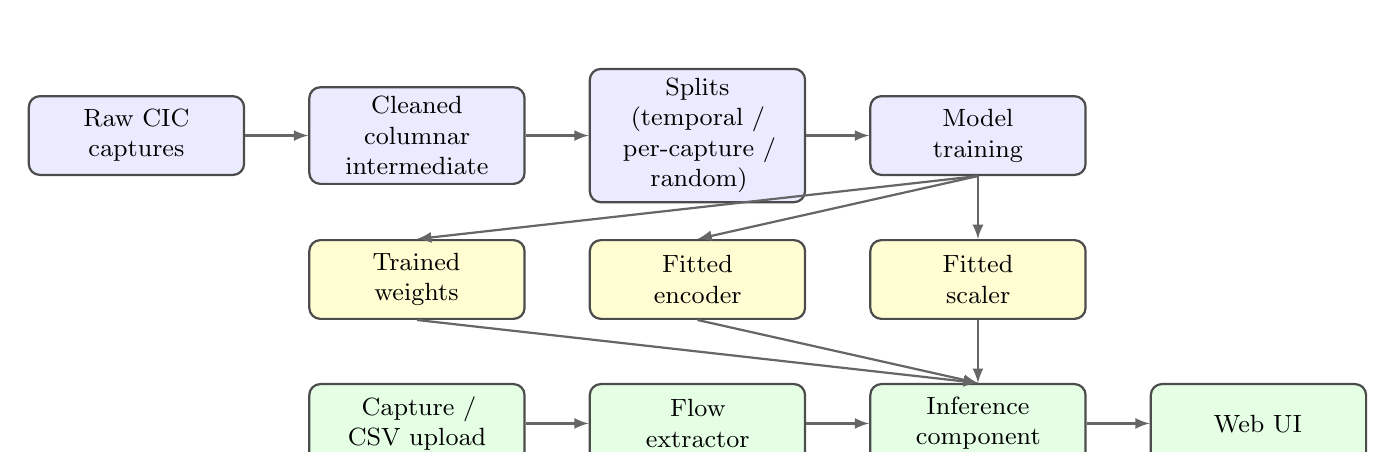
\begin{tikzpicture}[
        node distance=0.6cm and 0.8cm,
        layer/.style={
            rectangle,
            rounded corners=4pt,
            draw=black!70,
            thick,
            minimum width=2.6cm,
            minimum height=1.0cm,
            text width=2.5cm,
            align=center,
            font=\small
        },
        train/.style={layer, fill=blue!8},
        artefact/.style={layer, fill=yellow!18, minimum width=2.4cm},
        serve/.style={layer, fill=green!10},
        arrow/.style={
            ->,
            >=latex,
            thick,
            black!60
        }
    ]
    % Training pipeline (top row)
    \node[train] (raw)        {Raw CIC\\captures};
    \node[train, right=of raw]        (parquet)   {Cleaned\\columnar\\intermediate};
    \node[train, right=of parquet]    (split)     {Splits\\(temporal /\\per-capture /\\random)};
    \node[train, right=of split]      (train)     {Model\\training};

    % Artefact layer (middle)
    \node[artefact, below=of train, yshift=-0.2cm] (scaler)  {Fitted\\scaler};
    \node[artefact, left=of scaler]                (encoder) {Fitted\\encoder};
    \node[artefact, left=of encoder]               (weights) {Trained\\weights};

    % Serving pipeline (bottom row)
    \node[serve, below=of weights, yshift=-0.2cm]  (pcap)    {Capture /\\CSV upload};
    \node[serve, right=of pcap]                    (cic)     {Flow\\extractor};
    \node[serve, right=of cic]                     (predict) {Inference\\component};
    \node[serve, right=of predict]                 (gradio)  {Web UI};

    % Arrows: training row
    \draw[arrow] (raw) -- (parquet);
    \draw[arrow] (parquet) -- (split);
    \draw[arrow] (split) -- (train);

    % Train -> artefacts
    \draw[arrow] (train.south) -- (scaler.north);
    \draw[arrow] (train.south) -- (encoder.north);
    \draw[arrow] (train.south) -- (weights.north);

    % Artefacts -> predictor
    \draw[arrow] (scaler.south) -- (predict.north);
    \draw[arrow] (encoder.south) -- (predict.north);
    \draw[arrow] (weights.south) -- (predict.north);

    % Serving row
    \draw[arrow] (pcap) -- (cic);
    \draw[arrow] (cic) -- (predict);
    \draw[arrow] (predict) -- (gradio);

    \end{tikzpicture}%
    }
    \caption{High-level architecture of the RT-IDS application. The training pipeline (blue) produces three serialised artefacts (yellow), which the serving pipeline (green) loads to answer per-flow classification requests.}
    \label{fig:system_architecture}
\end{figure}

\subsection{Technology Stack and Rationale}
\label{subsec:tech_stack}

\par The technology choices are driven by the requirements above. Table~\ref{tab:tech_stack} lists each concern, the selected technology, and the reason it was chosen over the obvious alternatives.

\begin{table}[htbp]
\begin{center}
\small
\begin{tabular}{|p{70pt}|p{82pt}|p{198pt}|}
\hline
\textbf{Concern} & \textbf{Choice} & \textbf{Rationale} \\
\hline
\hline
Tabular data wrangling & Lazy columnar engine, compressed columnar intermediates & Lazy scanning lets the multi-tens-of-millions-of-rows CSV corpus be deduplicated and subsampled without ever materialising it in memory; columnar storage with strong compression cuts disk usage and reload time. \\
\hline
Feature scaling & Robust scaler (median / IQR) & CIC features have heavy-tailed distributions (rate, IAT, total bytes); scaling by median and IQR is more stable than zero-mean / unit-variance scaling under such tails. \\
\hline
Label encoding & Integer label encoder & Compact and reversible; the inverse transform is needed at inference time to display human-readable labels. \\
\hline
Imbalance handling & Class-weighted cross-entropy & Combats severe imbalance without synthetic data; SMOTE and weighted batch sampling are rejected (Section~\ref{subsec:class_weighted_ce}). \\
\hline
Deep model & Two-hidden-layer MLP with batch normalisation and dropout & MLPs are the natural fit for fixed-length tabular inputs, train fast on CPU, and serve as the strong baseline expected by the IDS literature. \\
\hline
Tree baselines & Random Forest, gradient-boosted trees & Required to demonstrate that the deep model is not strictly worse than a tree, which is the first question committees ask about tabular tasks. \\
\hline
Capture $\to$ flow CSV & CICFlowMeter (the CIC team's reference tool) & Reimplementing flow aggregation in Python would risk subtle numerical drift between the live-demo features and the training distribution. \\
\hline
Demo UI & Gradio UI + FastAPI REST endpoint; React dashboard (NEURAL IDS) & Gradio serves the local tab interface; FastAPI exposes a REST endpoint consumed by the React frontend, which adds model cards, a confidence gauge, and session history. \\
\hline
Public exposure & Docker on Hugging Face Spaces; React on Vercel & Backend containerised and served via HF Spaces; React frontend on Vercel. No router configuration required; permanent HTTPS URL. \\
\hline
Reproducibility & Single deterministic seed propagated to every random source & Required by NFR-3. \\
\hline
\end{tabular}
\end{center}
\caption{Technology stack of the RT-IDS application and rationale for each choice.}
\label{tab:tech_stack}
\end{table}

\subsection{Constraints and Assumptions}
\label{subsec:constraints}

\par Several constraints and assumptions bound the work and are acknowledged in the methodology. The 39-feature public CSV release of CICIoT2023 is the only source of training data; the 46-feature variant used by some published comparisons was not available from the official UNB CIC distribution at the time of writing, and although it is mirrored on third-party platforms, its provenance and preprocessing differ, so numerical results are not directly comparable across the two feature sets. The dataset was captured in a smart-home testbed of 105 IoT devices, so generalisation to industrial control systems, medical IoT, or vehicular networks is not claimed. Its features come from headers and metadata only, so detection of heavily encrypted traffic and of application-layer web attacks (SQL injection, XSS, command injection) is expected to be weak; this follows from the transport-layer feature set rather than from a model defect and is discussed in the results chapter. The production serving target is a single-container backend on Hugging Face Spaces with a static Vercel frontend, so distributed serving, load balancing, and high availability are out of scope and the container's cold-start latency is tolerated. Authentication uses Supabase email/password to restrict access during the thesis period and to scope each user's history (FR-D7), limited to identity verification with no role-based permissions or audit logging, and per-user isolation is enforced by Postgres row-level security rather than in client code, while the local-development Gradio UI does not authenticate. Finally, the deployed model is the one trained offline by the pipeline; the demo does not adapt to feedback during a session.

\chapter{Application Design, Implementation and Testing}
\label{chap:design_implementation}

\par This chapter covers the design and implementation of the application specified in Chapter~\ref{chap:requirements} and the testing that verifies the core functionality (per-flow classification of submitted traffic). It is organised top-down, starting from the architectural breakdown, moving through each component's design and the implementation choices that turn it into running code, and finishing with the testing strategy and the functional acceptance evidence.

\section{Architectural Overview}
\label{sec:architecture_overview}

\par The system is split into a training subsystem (offline) and a serving subsystem (online), as introduced in Section~\ref{sec:system_specification}. The two are decoupled by a small, well-defined contract: a fixed number of serialised artefacts per trained model variant. This decoupling is deliberate. It lets the training side iterate freely (different splits, granularities, hyperparameters) without forcing changes to the serving code, and it lets the serving code stay tiny and observable.

\subsection{Component Decomposition}
\label{subsec:module_decomposition}

\par The application decomposes into five components, each with a single concern so that a fault is locatable, and the boundary between them is the artefact contract rather than a network protocol or in-process API, which lets the training side be re-run independently of any deployed serving instance and the serving side be reloaded by pointing it at a different artefact directory. The training pipeline handles ingestion, deduplication, per-class subsampling, splitting, scaler and encoder fitting, model training, evaluation, latency benchmarking, and artefact persistence. The inference component loads the scaler, encoder, and weights for a given (split, granularity) variant, preprocesses incoming feature rows, runs the model, and returns labelled predictions with confidences. The capture-to-CSV bridge locates a CICFlowMeter backend, runs it as a subprocess against a packet capture, and returns the path of the feature CSV it produces. The web application discovers the model variants on disk, exposes the user interface, routes uploads through the inference component, and formats the verdicts. Beneath all of these, the project specification fixes the invariants (feature set, split strategies, classification granularities, and modelling constraints) that bind every component.

\subsection{Artefact Contract}
\label{subsec:artefact_contract}

\par The serving subsystem consumes exactly three artefacts per model variant, produced by the training pipeline and read back by the inference component: the fitted feature scaler for the split (one per split, shared across granularities because the input feature space is identical regardless of label encoding), the fitted label encoder for the (split, granularity) pair (one per granularity, because the label set changes), and the trained model weights for that pair.

\par The artefact filenames encode both the split and the granularity in a uniform pattern. As a consequence, the web application can probe the artefact directory at startup, parse each filename, and instantiate one inference component per complete artefact triple it finds, with no hard-coded list of variants. Exposing a newly trained variant in the user interface is therefore purely a question of dropping its three files into the artefact directory and restarting the application.

\section{Data Pipeline Design}
\label{sec:data_pipeline_design}

\par The training data pipeline performs a sequence of deterministic transformations from the raw per-folder CSVs to the train/validation/test tensors that feed the model. Each transformation is a separate pipeline phase so that intermediate state is inspectable.

\subsection{Ingestion and Deduplication}
\label{subsec:ingestion}

\par For each of the attack folders, the pipeline lazily scans every CSV, projects only the feature columns plus a synthetic column that carries the source-capture filename, and concatenates the resulting lazy frames. Materialisation happens only after the projection, so the multi-tens-of-millions-of-rows corpus is never held in memory in its raw width.

\par CICIoT2023 contains a substantial fraction of exact duplicate rows, a known property of the dataset and a recurring concern in the literature. Deduplication is applied immediately after concatenation, before any sampling. Deduplicating before sampling is essential: a folder where most rows are duplicated would otherwise have the same row repeated many times in the sample, which would inflate accuracy on the corresponding test rows. The quantitative impact of each pipeline stage (raw count, duplicates removed, unique rows, sampling cap applied) is reported in Chapter~\ref{chap:results} (Figure~\ref{fig:ingest_waterfall}).

\subsection{Per-Class Subsampling}
\label{subsec:subsampling}

\par After deduplication, every folder whose deduplicated row count exceeds the per-class cap is randomly subsampled to that cap with a fixed seed. This brings the effective training-set size down from tens of millions of rows to a few million while keeping every attack class represented.

\par The cap is set at the high end of the range used in the CICIoT2023 literature. Random sampling is preferred over taking the leading rows of each folder because each attack folder is a chronological concatenation of several capture sessions: the first $N$ rows come almost entirely from the first session, and a leading-rows sample would bias the model toward whatever happened in that opening session.

\subsection{Caching}
\label{subsec:caching}

\par The deduplicated, subsampled, labelled rows are concatenated across folders and written to a single Zstandard-compressed columnar file. Subsequent runs skip ingestion and load from this cache directly. Regeneration is forced by deleting the cache file. This is documented inline so future runs do not silently use a stale cache after sampling logic changes.

\subsection{Cleaning}
\label{subsec:cleaning}

\par The cleaning phase performs three operations on the materialised frame. First, null-label rows are dropped (defensive only; labels come from folder names, so this should be a no-op). Second, infinities are replaced with nulls; the actual median imputation is deferred to after the train/validation/test split so the medians are computed on the training partition only. Third, a $\log(1+x)$ transform is applied to the heavy-tailed continuous features (rates, total bytes, inter-arrival times). Binary protocol and flag indicators are excluded from the log transform.

\subsection{Three Split Strategies}
\label{subsec:split_strategies}

\par Three splitting functions are defined and selected by configuration. Their design follows directly from the requirements in Section~\ref{subsec:pipeline_requirements}.

\par \textbf{Random row split.} Two stratified splits in series produce 70/15/15 train/validation/test partitions, stratified by the fine-grained label so every class appears in every partition. This is reported only for parity with previously published numbers.

\par \textbf{Per-capture split.} Two consecutive group-aware splits with the source-capture filename as the group identifier produce a 70/15/15 split where no source capture ever appears in more than one partition. This eliminates within-session redundancy leaking across the boundary, but preserves no temporal order.

\par \textbf{Temporal split (headline).} For each attack folder, the source captures are sorted by filename and partitioned chronologically: the earliest 70\% become train, the next 15\% become validation, and the latest 15\% become test. Folders with fewer than three distinct source captures fall back to a row-level temporal split inside the folder. This mirrors deployment (train on past, test on future) and is the headline result reported in the thesis. The temporal F1 is expected to sit a few points below the random F1; that gap is the honest generalisation story.

\subsection{Train-Only Preprocessing Fit}
\label{subsec:train_fit_preprocess}

\par For each split, column medians are computed on the training rows only, nulls in the train, validation, and test partitions are imputed using those medians, and the robust scaler is fitted on training rows alone before being applied to all three partitions. The robust scaler standardises each feature by its median and interquartile range rather than its mean and standard deviation:
\begin{equation}
    x' = \frac{x - \operatorname{median}(x)}{\mathrm{IQR}(x)}, \qquad \mathrm{IQR}(x) = Q_3(x) - Q_1(x),
    \label{eq:robust_scaler}
\end{equation}
where $Q_1$ and $Q_3$ are the first and third quartiles estimated on the training rows. Centring on the median and dividing by the IQR makes the transform insensitive to the heavy upper tails of the CIC rate and byte-count features, which would otherwise dominate a mean/variance scaler. The contract that medians, quartiles, and the scaler are fitted strictly on training rows enforces NFR-3 (no test-set leakage) and is what makes the temporal-split metrics meaningful.

\section{Model Architecture and Training}
\label{sec:model_architecture}

\subsection{MLP Topology}
\label{subsec:mlp_topology}

\par The model is a two-hidden-layer multi-layer perceptron with batch normalisation and dropout:

\begin{equation*}
    n_{\text{features}} \xrightarrow{\text{Linear}} 128 \xrightarrow{\text{BN, ReLU, Dropout}_{0.3}} 64 \xrightarrow{\text{BN, ReLU, Dropout}_{0.3}} n_{\text{classes}}
\end{equation*}

\par Batch normalisation, applied after each hidden linear layer, standardises that layer's pre-activations across the mini-batch to zero mean and unit variance before rescaling them by two learned parameters $(\gamma, \beta)$:
\begin{equation}
    \mathrm{BN}(z) = \gamma \, \frac{z - \mu_{\mathcal{B}}}{\sqrt{\sigma_{\mathcal{B}}^2 + \epsilon}} + \beta,
    \label{eq:batchnorm}
\end{equation}
where $\mu_{\mathcal{B}}$ and $\sigma_{\mathcal{B}}^2$ are the per-feature mean and variance over the current batch $\mathcal{B}$ and $\epsilon$ is a small constant for numerical stability.

\par The architecture is intentionally small. Three considerations drive this choice. First, every empirical study of MLPs on tabular data has reported diminishing returns past two hidden layers when the input dimensionality is in the tens. Second, batch normalisation (Equation~\ref{eq:batchnorm}) is required to stabilise training under large class-weight swings: at the fine-grained granularity, the heaviest class weight is more than fifty times the lightest, and gradients without batch normalisation would oscillate. Third, the 0.3 dropout rate is a deliberately conservative regularisation choice that empirically generalises better than the more common 0.5 on this dataset, where the cleaned training set is already several million rows.

\subsection{Class-Weighted Cross-Entropy}
\label{subsec:class_weighted_ce}

\par Class weights are computed using the standard balanced-frequency rule applied to the encoded training labels, then passed to the cross-entropy loss. For a problem with $K$ classes, $N$ training samples, and $n_c$ samples in class $c$, the weight of class $c$ is
\begin{equation}
    w_c = \frac{N}{K \, n_c},
    \label{eq:balanced_weights}
\end{equation}
so that rare classes receive proportionally larger weight (and $\sum_c n_c w_c = N$). These weights enter the multi-class cross-entropy loss applied to the softmax outputs $\hat{y}_{i,k}$:
\begin{equation}
    \mathcal{L} = -\frac{1}{N} \sum_{i=1}^{N} \sum_{k=1}^{K} w_{k}\, y_{i,k} \log\!\big(\hat{y}_{i,k}\big),
    \label{eq:weighted_ce}
\end{equation}
where $y_{i,k}$ is the one-hot ground-truth indicator for sample $i$ and class $k$. Equation~\eqref{eq:weighted_ce} is the multi-class, class-weighted generalisation of the binary cross-entropy in Equation~\eqref{eq:bce_loss}. Weighting is preferred over resampling because SMOTE would generate synthetic flow vectors that have no operational meaning (a half-and-half SYN-flood / DNS-spoofing flow does not correspond to any real attack), and weighted batch sampling would be redundant with weighted cross-entropy.

\subsection{Optimiser, Schedule, and Early Stopping}
\label{subsec:training_loop}

\par Training uses Adam with an initial learning rate of $10^{-3}$, paired with a learning-rate schedule that halves the rate after two consecutive epochs without validation-loss improvement. A separate early-stopping mechanism with a patience of five epochs caps total training. The batch size is 4096, large enough to amortise the batch-normalisation overhead and small enough to keep the per-step gradient meaningful.

\par The training loop tracks training loss, validation loss, and the current learning rate per epoch, restoring the best validation-loss state at the end. The best state is what is serialised; the final-epoch state is discarded.

\subsection{Hyperparameter Selection}
\label{subsec:hpo}

\par The architecture and optimisation settings above are not arbitrary: they were selected by an automated hyperparameter search rather than fixed by hand. A Tree-structured Parzen Estimator (TPE) sampler explores the search space summarised in Table~\ref{tab:hpo_space} over fifteen trials, each trained for ten epochs on a 100{,}000-row stratified subsample of the training set, with a median pruner terminating clearly unpromising trials early. The objective minimised is the validation loss. The search confirmed that a compact two-hidden-layer network with $[128, 64]$ units, $0.3$ dropout, ReLU activations, the Adam optimiser, and a $4096$ batch size is a strong configuration for this dataset; this configuration is then retrained to convergence (up to fifty epochs with early stopping) on the full training set and used for all reported results.

\begin{table}[htbp]
\begin{center}
\begin{tabular}{|p{120pt}|p{200pt}|}
\hline
\textbf{Hyperparameter} & \textbf{Search range} \\
\hline
\hline Hidden layers & 2--4 \\
\hline Units per layer & 64--512 (step 32) \\
\hline Dropout & 0.1--0.5 \\
\hline Activation & ReLU, ELU, LeakyReLU \\
\hline Learning rate & $10^{-4}$--$10^{-2}$ (log scale) \\
\hline Optimiser & Adam, AdamW \\
\hline Batch size & 2048, 4096, 8192 \\
\hline
\end{tabular}
\end{center}
\caption{Optuna TPE search space for the MLP. Fifteen trials, ten epochs each on a 100{,}000-row subsample, validation loss as the objective, median pruning.}
\label{tab:hpo_space}
\end{table}

\section{Inference Component Design}
\label{sec:inference_layer}

\par The inference component is the single seam between trained artefacts and live requests. Its constructor takes the artefact directory, the split name, and the granularity, and loads the matching triple. Its prediction method takes a frame of feature rows and returns the predicted labels, the per-prediction confidences, the full softmax probabilities, and the class-name list in the encoder's index order.

\subsection{Preprocessing Mirror}
\label{subsec:preprocessing_mirror}

\par The trickiest part of the inference component is matching the training-time preprocessing exactly, and three rules in its preprocessing path each mirror a training-time decision. The expected feature columns are validated and reordered so that column ordering does not silently shift between the trained scaler and the live data. Infinities are replaced with nulls and the $\log(1+x)$ transform is applied to the continuous features only, leaving the flag and protocol indicators binary. Residual nulls are then filled with zeros: at training time median imputation handled nulls, but the trained scaler operates in the transformed space, so a residual null in a live request is filled with a constant rather than a re-derived median. The transformed array is passed through the scaler's transform method, never a re-fit, since the scaler is immutable at inference time.

\subsection{Confidence and Label Decoding}
\label{subsec:confidence_decoding}

\par The model emits logits; a softmax along the class dimension produces per-class probabilities; the argmax selects the predicted class index; the encoder's inverse transform maps the index back to the human-readable label. The maximum softmax probability is reported as confidence. Confidence here is not a calibrated probability; it is reported because end users (committee, presenter) intuitively expect a number alongside each verdict, and the maximum softmax is the cheapest reasonable proxy.

\section{Capture-to-CSV Bridge Design}
\label{sec:cicflowmeter_design}

\par The bridge component exists for one reason: the training data was derived from an established flow extractor, so the project must not reimplement flow extraction in Python, on pain of subtle numerical drift between the live and training distributions. The component wraps two backends and returns the path of the feature CSV. The Java CICFlowMeter is preferred, detected through an environment variable pointing at a built installation and invoked through the launcher script for the host platform (one variant for Linux and macOS, one for Windows). If it is absent, the bridge falls back to a community Python port located through the executable search path, and if neither is available it raises an error naming both options. The two backends differ in output filename convention, so the bridge renames the produced file to a single canonical form and downstream code never branches on backend. Both are launched with their standard output and error captured, and a non-zero exit is translated into a domain-level error carrying that standard error, which is what surfaces under FR-D4 as the tool's own diagnostic message rather than a Python traceback.

\section{Web Application Design}
\label{sec:webapp_design}

\par The serving subsystem is implemented as two cooperating layers: a \textbf{backend} (Gradio UI combined with a FastAPI REST endpoint, running in a single Python process) and a \textbf{React dashboard frontend} that calls the REST endpoint and provides a richer user experience. The two layers are decoupled through the REST API contract, which allows the frontend to be hosted independently on a public platform while the backend runs locally or on Hugging Face Spaces.

\subsection{Backend: Gradio + FastAPI}
\label{subsec:backend_gradio_fastapi}

\par At startup, the backend performs the filesystem-driven discovery described in Section~\ref{subsec:artefact_contract}: it globs the artefact directory for trained model weights, attempts to load each complete artefact triple, and builds a dictionary of ready predictors keyed by a human-readable \texttt{split / granularity} string. If no triples are found, the process exits with a diagnostic message.

\par The backend exposes two interfaces over the same port. The Gradio interface provides a lightweight local UI with a model-variant dropdown and two upload tabs (one for pre-extracted CSVs, one for raw packet captures). The FastAPI REST endpoint at \texttt{/api/classify} accepts a multipart form submission with the upload file, a model type label, the split name, the classification mode, and the input type (CSV or PCAP). It runs the prediction and returns a JSON response carrying the top label, confidence score, full per-class probability vector, per-flow breakdown, and processing time in milliseconds. Both interfaces share the same predictor pool and the same capture-to-CSV bridge, so they are functionally equivalent.

\subsection{Frontend: NEURAL IDS React Dashboard}
\label{subsec:frontend_react}

\par The React frontend connects to the REST endpoint and presents a polished cyberpunk-themed dashboard under the branding \emph{NEURAL IDS}. Its main screen (Figure~\ref{fig:app_dashboard}) presents three model-selection cards (MLP Neural Network, Random Forest, XGBoost) that set the \texttt{model\_type} field of subsequent API calls, and an analysis history table that persists the timestamp, model label, filename, dominant predicted class, and confidence of every classification run, scoped to the signed-in user and retained across sessions (Section~\ref{subsec:auth_persistence}).

\par On submission, the frontend calls \texttt{POST /api/classify} with the selected model type, split, and mode parameters. The backend routes the request through the corresponding artefact triple and returns the prediction result. The frontend renders the result on a dedicated analysis screen (Figure~\ref{fig:app_attack}) displaying a confidence gauge, a ranked probability bar chart for all classes, per-request metadata (model, mode, split, flow count, processing time), and a flow-count breakdown by predicted label.

\subsection{Two Symmetric Upload Paths}
\label{subsec:two_tabs}

\par The CSV and PCAP upload paths are symmetric at the API level. Both paths reach the same inference component after the optional flow-extraction step. The CSV path validates column presence and forwards the frame directly; the PCAP path materialises the capture in a temporary directory, invokes the CICFlowMeter bridge to produce a feature CSV, and then takes the same downstream route. This shared post-extraction path means the JSON response schema and the frontend rendering logic are identical for both input types.

\subsection{Authentication and Result Persistence}
\label{subsec:auth_persistence}

\par The deployed frontend communicates with two independent backends, and that separation is the central design decision of the serving tier (Figure~\ref{fig:deployment_topology}). The first is the \emph{stateless inference channel}: the React single-page application issues a cross-origin \texttt{POST /api/classify} to the FastAPI endpoint on Hugging Face Spaces (Section~\ref{subsec:backend_gradio_fastapi}) and receives a JSON verdict. That backend holds no database and retains nothing about the user between requests. It is the artefact-driven predictor described throughout this chapter, merely reached over HTTPS. The second is the \emph{stateful identity-and-history channel}: the same application talks directly to a managed Supabase project for authentication and for persisting the user's past results. Inference and identity are therefore fully decoupled: either backend can be replaced without touching the other, and an inference request never blocks on the persistence layer.

\par Authentication uses Supabase's email/password provider. On sign-in the client receives a JSON Web Token that is attached to subsequent storage requests, and the session is restored on reload from the persisted token. After each classification, the results screen writes a single row into the \texttt{analyses} table, tagged with the authenticated user's identifier, and the dashboard reads the same table back to render the history list. Each row holds only derived result metadata, never the uploaded capture or CSV: a surrogate UUID key, the owning \texttt{user\_id}, a server-side timestamp, the classifier variant and classification granularity, the input modality (CSV or packet capture), the uploaded file name, the dominant predicted label with its calibrated confidence, and the full per-class probability vector as JSON. This keeps the persistence tier consistent with FR-D5. Per-user isolation is not enforced in client code: a row-level-security policy restricts every \texttt{select} and \texttt{insert} to rows whose \texttt{user\_id} matches the caller's authenticated identifier, so one user can never read another's history even though all rows share a single table.

\subsection{Public Deployment}
\label{subsec:public_deployment}

\par The backend is packaged as a Docker image and deployed on Hugging Face Spaces, allowing the demo to be reached from any browser without the presenter's local machine being reachable. The React frontend is deployed separately on Vercel and communicates with the Spaces backend over HTTPS. For the local defence demonstration, the same backend process is run directly on the presenter's laptop and reached through the loopback address, with the Gradio tab serving as the fallback UI.

\par Figure~\ref{fig:deployment_topology} shows the resulting runtime topology. Vercel delivers the built single-page application to the browser; at runtime the application fans out to the two decoupled backends of Section~\ref{subsec:auth_persistence}. The diagram makes the key property explicit: the inference path (browser~$\leftrightarrow$~Hugging Face Spaces) and the identity-and-history path (browser~$\leftrightarrow$~Supabase) share no server-side state and can fail or be replaced independently.

\begin{figure}[htbp]
    \centering
    \resizebox{0.82\textwidth}{!}{%
    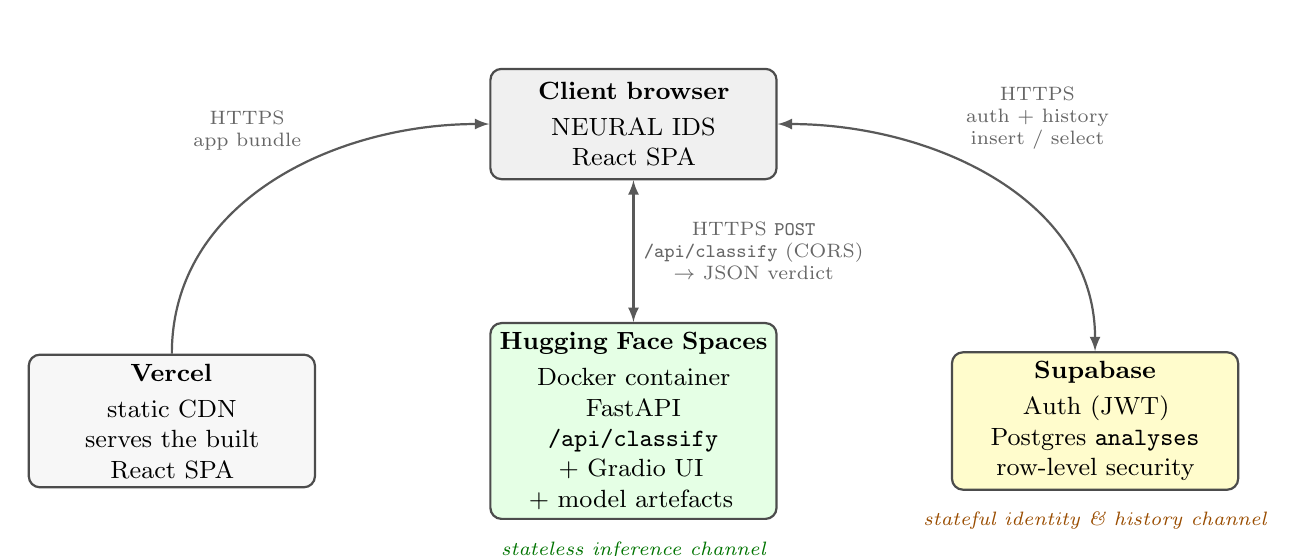
\begin{tikzpicture}[
        node distance=1.8cm and 2.2cm,
        box/.style={
            rectangle, rounded corners=4pt, draw=black!70, thick,
            minimum width=3.2cm, minimum height=1.4cm, text width=3.4cm,
            align=center, font=\small
        },
        client/.style={box, fill=gray!12},
        edge/.style={box, fill=gray!6},
        infer/.style={box, fill=green!10},
        store/.style={box, fill=yellow!20},
        arrow/.style={->, >=latex, thick, black!65},
        biarrow/.style={<->, >=latex, thick, black!65},
        lbl/.style={font=\scriptsize, black!60, align=center}
    ]
    % Client (top)
    \node[client] (browser) {\textbf{Client browser}\\[2pt] NEURAL IDS\\ React SPA};

    % Infrastructure row (bottom)
    \node[infer, below=of browser]      (hf)     {\textbf{Hugging Face Spaces}\\[2pt] Docker container\\ FastAPI \texttt{/api/classify}\\ + Gradio UI\\ + model artefacts};
    \node[edge, left=of hf]             (vercel) {\textbf{Vercel}\\[2pt] static CDN\\ serves the built\\ React SPA};
    \node[store, right=of hf]           (supa)   {\textbf{Supabase}\\[2pt] Auth (JWT)\\ Postgres \texttt{analyses}\\ row-level security};

    % Delivery of the SPA
    \draw[arrow] (vercel.north) to[out=90, in=180]
        node[lbl, above left, pos=0.6] {HTTPS\\ app bundle} (browser.west);

    % Stateless inference channel
    \draw[biarrow] (browser.south) -- node[lbl, right] {HTTPS \texttt{POST}\\ \texttt{/api/classify} (CORS)\\ $\rightarrow$ JSON verdict} (hf.north);

    % Stateful identity + history channel
    \draw[biarrow] (browser.east) to[out=0, in=90]
        node[lbl, above right, pos=0.4] {HTTPS\\ auth + history\\ insert / select} (supa.north);

    % Channel annotations
    \node[lbl, below=0.15cm of hf, green!45!black] {\itshape stateless inference channel};
    \node[lbl, below=0.15cm of supa, orange!60!black] {\itshape stateful identity \& history channel};

    \end{tikzpicture}%
    }
    \caption{Runtime deployment topology of the serving subsystem. Vercel delivers the static React SPA (grey); at runtime the SPA drives two independent backends: a \emph{stateless} inference service on Hugging Face Spaces (green) reached via \texttt{POST /api/classify}, and a \emph{stateful} Supabase project (yellow) for authentication and per-user history. The two channels share no server-side state, so inference never blocks on persistence and either tier can be replaced in isolation.}
    \label{fig:deployment_topology}
\end{figure}

\section{Implementation Notes}
\label{sec:implementation_details}

\par Several implementation choices turn the design above into running code that respects the resource budgets. Memory discipline follows from the 16~GB budget (NFR-4): lazy frames are used wherever ingestion touches raw CSVs, with materialisation deferred until after column projection; the deduplicated, subsampled frame is the only materialised object on the data side, and its memory is reclaimed once it has been converted to numpy arrays, before the training tensors are allocated; and the cached intermediate is the only persistent caching boundary, with no in-memory cache surviving a restart. Determinism follows from broadcasting a single seed to every random source, the numerical library, the deep-learning framework on CPU and GPU, the framework's deterministic backend flags, and the dataset samplers, so re-running against the same source files reproduces metrics within the few-thousandths-of-an-F1-point tolerance of NFR-3.

\par The remaining notes concern operability. The pipeline prints concise progress at every phase (per-folder ingestion counts, per-split row counts, missing-class warnings, per-epoch losses, and final per-class metrics) and renders training curves and confusion matrices inline, while the web application prints only its bind address and any per-request error. Configuration lives in a small block of named constants near the top of the notebook (the per-class cap, the active splits and granularities, the batch size, the maximum epochs, the early-stopping patience, the learning rate, and the seed), with a quick iteration mode (one split, one granularity) and a full thesis-run mode documented alongside so iteration cost is predictable. The runtime dependencies stay within the standard scientific-Python stack (a lazy columnar engine, a deep-learning framework, a tabular machine-learning library, and plotting libraries) plus a lightweight web-UI framework and a gradient-boosted-trees implementation for the baselines; there is no serving framework, since the demo loads the model directly into the application process, and no packaging beyond a flat directory launched by a single command, which satisfies NFR-7.

\section{Testing Strategy}
\label{sec:testing_strategy}

\par The application is tested at three levels: shape-and-determinism sanity checks inside the training pipeline; integration smoke tests over each (split, granularity) artefact triple; and the functional acceptance test, which demonstrates the core functionality end-to-end.

\subsection{Pipeline-Level Sanity Checks}
\label{subsec:notebook_sanity}

\par The training pipeline contains assertions and printed sanity checks at every transition. An assertion confirms that the fine-grained label mapping covers every attack folder exactly once, guarding against a missing or duplicated entry, and a second assertion during ingestion confirms that no folder is left unmapped, guarding against a new attack folder being silently dropped. For each split, a check confirms that every fine-grained label appears at least once in the train partition, flagging any missing class with a warning. Per-folder row counts (raw, deduplicated, sampled) are printed during ingestion, so a sudden mismatch between the raw and deduplicated counts is an immediate cue that the source data has changed.

\subsection{Artefact Round-Trip Test}
\label{subsec:roundtrip_test}

\par For every (split, granularity) pair, after training, the pipeline reloads the freshly written artefacts using the exact code path the demo uses and predicts on the test partition. The reloaded predictions are compared against the in-memory predictions of the still-loaded model. The two must agree exactly. This test caught two real bugs during development: a column-ordering drift between training and inference, and a silent dtype mismatch when arrays were converted to tensors without an explicit precision cast.

\subsection{Latency Benchmark}
\label{subsec:latency_benchmark}

\par For each trained model, the benchmark loop runs $10{,}000$ inference passes per batch size in $\{1, 32, 256, 1024\}$ on CPU after a warmup of one hundred passes, with the timer wrapped around the feature scaling step \emph{and} the model forward pass. The pipeline reports the p50, p95, and p99 of the per-batch latency in milliseconds and the implied flows-per-second throughput. NFR-1 (sub-100~ms p95 end-to-end on a consumer laptop CPU at any of those batch sizes) is the acceptance criterion.

\subsection{Functional Acceptance Test: Capture to Verdict}
\label{subsec:f1_functional_test}

\par The core functionality is verified end-to-end with two test inputs whose ground-truth labels are known, so the test is a binary pass/fail rather than a subjective inspection. Each test runs the demo, uploads the input, and reads the predicted-label distribution. The benign baseline is a short capture of normal browsing traffic produced on the demo machine, and it passes if at least 95\% of flows are predicted Benign at the binary granularity. The synthetic flood is a capture of a SYN-flood attack against a local target generated with a standard packet-crafting tool, and it passes if at least 95\% of flows are predicted Attack at the binary granularity and the dominant predicted family is DDoS at the attack-family granularity.

\par These thresholds are deliberately set well below the test-set numbers (which are typically 0.97+ in the binary case) so the test tolerates the inevitable distribution shift between the training data and the live demo machine, while still failing loudly if the model has been deployed against a wrong scaler or a wrong encoder.

\subsection{Negative-Path Testing}
\label{subsec:negative_path_testing}

\par Three negative scenarios are exercised manually from the public component surface, so they reproduce from a brief interactive session. Uploading a CSV missing one or more expected feature columns should produce a domain-level error naming the missing columns, surfaced as the summary message with an empty table, which verifies FR-D4. Uploading a non-capture file (for example a text file renamed to a capture extension) should produce a flow-extraction error carrying the tool's stderr, again surfaced as the summary message, which also verifies FR-D4. Running the demo with no artefacts on disk should exit quickly with a message pointing the user back to the training pipeline, which verifies graceful behaviour when discovery yields nothing (FR-D2).

\section{Deployment and Runtime Behaviour}
\label{sec:deployment_runtime}

\par The serving subsystem runs as a single Python process inside the project's virtual environment. The packet-capture path additionally needs a CICFlowMeter backend reachable from the process, either the Java reference implementation located through the \texttt{CICFLOWMETER\_HOME} environment variable or the Python community port located through the executable search path, whereas the CSV path needs neither, since CICFlowMeter has already been applied upstream. On startup the application runs the discovery probe of Section~\ref{subsec:backend_gradio_fastapi}, populates the variant dropdown with every artefact triple on disk, and defaults to the first one returned; the temporal-split binary variant is the one used for the acceptance evidence in Section~\ref{sec:f1_acceptance_evidence}, and the dropdown lets the same input be re-classified under any other variant. A request then follows one of two symmetric paths that converge on the same downstream code: the CSV path reads the file and validates it against the expected columns, while the packet-capture path materialises the \texttt{.pcap} or \texttt{.pcapng} file in a temporary directory and invokes the capture-to-CSV bridge to produce a feature CSV. In both cases the response is a summary line of the form \enquote{$N$ flows classified, LabelA: $n_A$ | LabelB: $n_B$ | $\dots$} sorted by descending count, together with a per-flow verdict table giving the row index, the predicted label, and the maximum-softmax confidence to four decimal digits. Response time is dominated by flow extraction on the packet-capture path and by scaler-plus-forward latency on the CSV path, both of which fall inside the NFR-1 budget for the captures used as acceptance evidence.

\section{Functional Acceptance Evidence}
\label{sec:f1_acceptance_evidence}

\par The functional acceptance test specified in Section~\ref{subsec:f1_functional_test} was executed against the deployed serving subsystem using both the local Gradio interface and the NEURAL IDS React dashboard. Two pre-extracted feature CSVs with known ground-truth labels were submitted: \texttt{demo\_benign.csv} (normal browsing traffic captured on the demo machine and converted to CIC features) and \texttt{demo\_syn\_flood.csv} (a SYN-flood attack directed at a local target, converted via the same flow-extraction tool). Figure~\ref{fig:app_dashboard} shows the NEURAL IDS dashboard after all four acceptance runs have been completed, with the full analysis history visible in the main panel.

\par The history confirms both halves of the acceptance criterion. For \texttt{demo\_syn\_flood.csv}, the binary temporal-split MLP labelled every flow (100\%) as Attack with a mean calibrated confidence of 99.6\%, and a subsequent run of the same file under the 8-class variant confirmed DoS as the dominant family, both correct. For \texttt{demo\_benign.csv}, the binary MLP returned Benign on 98\% of flows (mean dominant-class confidence 71.9\%), so the fraction labelled Benign exceeds the 95\% threshold defined in Section~\ref{subsec:f1_functional_test}, discharging the no-false-alarm half of the criterion. (Confidence values report the mean softmax probability of the dominant class after temperature scaling, not the fraction of flows in that class.)

\begin{figure}[htbp]
    \centering
    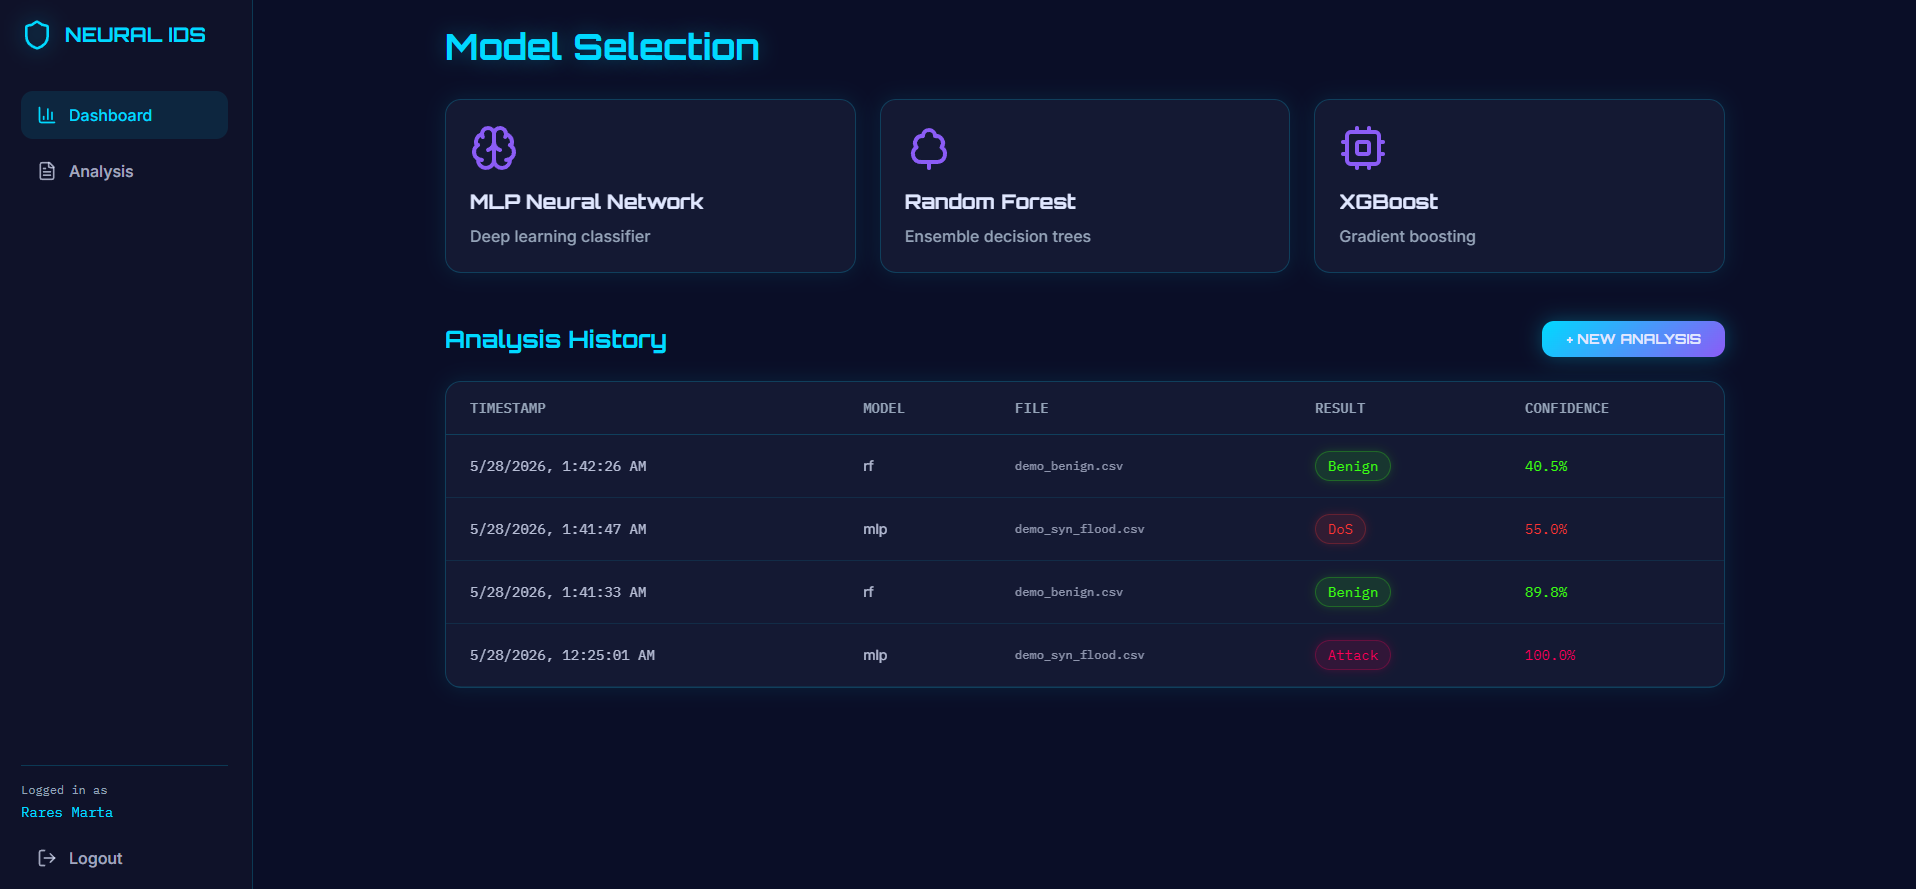
\includegraphics[width=0.78\textwidth]{figures/app_dashboard.png}
    \caption{NEURAL IDS dashboard after the acceptance runs. The analysis history table records four classification requests: the SYN-flood capture classified as Attack (near-certain binary confidence) and as DoS ($\approx$55\%) under different granularities, and the benign capture classified as Benign. The three model-selection cards at the top set the \texttt{model\_type} field of subsequent API calls. (Screenshot is illustrative; binary confidence is reported after temperature scaling in the text.)}
    \label{fig:app_dashboard}
\end{figure}

\par Figure~\ref{fig:app_attack} shows the detailed result screen for the SYN-flood capture classified under the temporal-split 8-class Random Forest variant. The top predicted class is \textbf{DoS} at 55\% mean confidence, with \textbf{DDoS} as the second-ranked class at 45\%. This is the expected result: a SYN flood is structurally a single-source volumetric attack, which the model correctly places in the DoS family (single-source high-rate flood) rather than DDoS (distributed multi-source flood). The processing time of 8~ms for 50 flows is well within the NFR-1 budget of 100~ms at p95.

\begin{figure}[htbp]
    \centering
    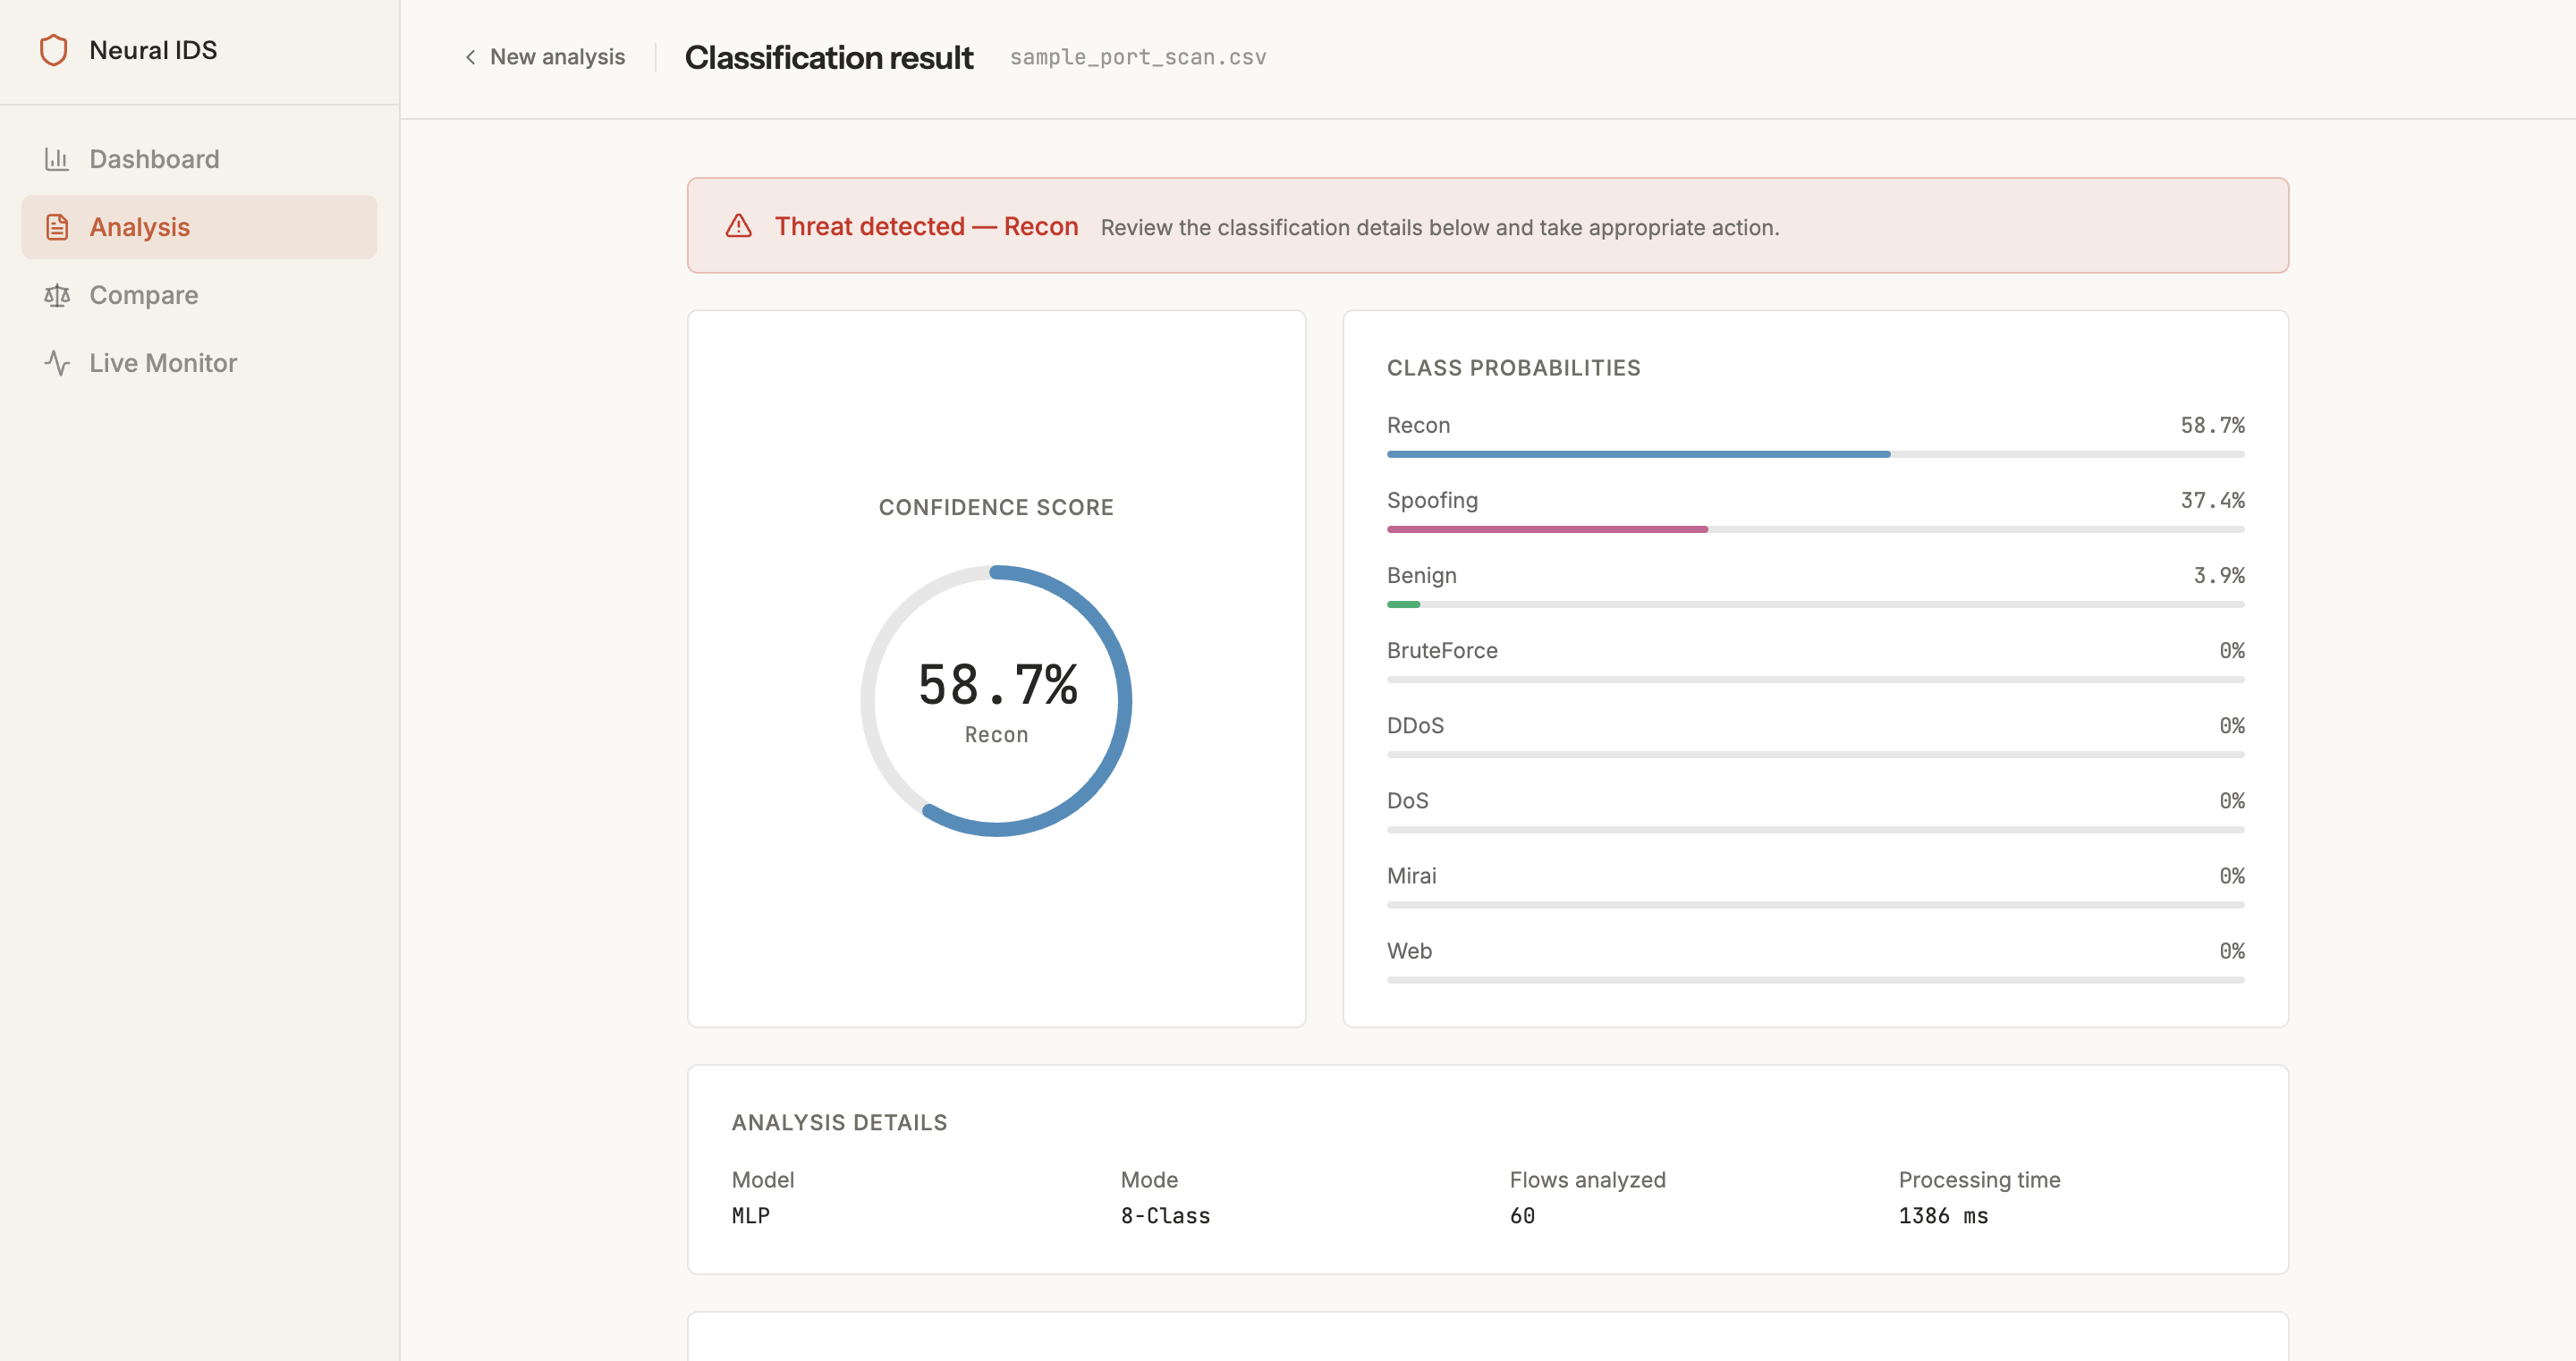
\includegraphics[width=0.50\textwidth]{figures/app_attack.png}
    \caption{Functional acceptance: SYN-flood capture classified under the temporal-split 8-class Random Forest variant. The alert banner confirms a threat detection; the class-probability panel ranks DoS (55\%) above DDoS (45\%), correctly identifying the single-source flood family. Analysis metadata (50 flows, 8~ms processing time) are shown in the lower panel.}
    \label{fig:app_attack}
\end{figure}

\chapter{Results and Discussion}
\label{chap:results}

\par This chapter will report experimental results across the three split strategies and the three classification granularities, the comparison against tree-based baselines (Random Forest, XGBoost), the latency benchmark, and a discussion of per-attack-family detection performance --- with particular attention to the expected weaker detection of web-family attacks. (To be completed in a subsequent assignment.)


\chapter{Conclusions and Future Work}
\label{chap:conclusions}

\par This chapter will summarize the findings of the thesis and outline directions for future work. (To be completed in a subsequent assignment.)

%\addcontentsline{toc}{chapter}{Conclusions}
\nocite{*}
\bibliographystyle{plain}
\bibliography{references}

\end{document}